\documentclass{article}
\usepackage{graphicx}
\usepackage{booktabs}
\usepackage{parskip}
\usepackage{tcolorbox}
\usepackage[fleqn]{amsmath}
\usepackage{multicol}
\usepackage{amsmath}
\usepackage{multicol}
\usepackage{float}
\usepackage{amssymb}
\usepackage{gensymb}
\usepackage[inline]{enumitem}
\usepackage{titling}
\usepackage[margin=0.5in]{geometry}
\setlength{\droptitle}{-1in}
\usepackage{array}
\usepackage{amsmath}
\usepackage{natbib}
\usepackage{hyperref}
\newcommand{\commandnote}[1]{
    \begin{tcolorbox}[
        standard jigsaw,
        title=Note,
    ]
        #1
    \end{tcolorbox}
}
\newcommand{\minititle}[1]{
\subsubsection*{#1}
}

\title{\vspace{1ex} Data Eng. Notes \vspace{-1ex}}
\author{ibrahim.nasser@fau.de}
\date{}
\begin{document}
\maketitle
\section*{Disclaimer}

These are my personal notes and are not official course documents. They may contain inaccuracies or omissions, hence, they should not be considered as a substitute for official course materials or as comprehensive preparation for examinations.

\tableofcontents

\clearpage
\section{Introduction and Basic Data Types}
We call the data \textbf{Tabular} when there are no modelled dependencies between attributes, for example, demographic attributes such as age, gender, ZIP code, etc. (also called \textit{Nondependency-Oriented Data}). Otherwise it is \textbf{Non-Tabular}, e.g. social networks, time series, etc.

\textbf{Matrix Representation of Data}

A set  $X = \{ X_i \mid  i \in \{1 \dots n \}\}, $ with $n$ records (samples) is a $d$-dimensional dataset iff each sample $X_i$ is a set of $\{ x_j \mid j \in \{ 1 \dots d\} \}$ attributes (features). $X$ is tabular if it is invariant w.r.t shuffling of samples and features. Each feature $x_j$ has its own domain $\mathcal{D}_j$

\mydef{Quantitative vs. Categorical}{A variable $x$ is quantitative (numeric) if its domain $\mathcal{D}_x$ is numeric. Otherwise, Categorical.
\textit{Examples (Q): }age, weight, height, BMI, Date of Birth.
\textit{Examples (C): }name, gender, country, ZIP Code, weather, ID, day.}

\mydef{Nominal vs. Ordinal}{A categorical variable $x$ is ordinal if its domain $\mathcal{D}_x$ has a natural ordering. Otherwise, Nominal.
\textit{Examples (N): }weather, name, gender, country, ZIP, ID, day
\textit{Examples (O): }heat level, textual gpa.}

\mydef{Finite vs. Infinite}{A variable $x$ has a finite domain iff $|\mathcal{D}_x| = N , N \in \mathbb{N}$. Otherwise, Infinite.
\textit{Examples (F): }age (years), country, ZIP, ID, gender, day.
\textit{Examples (I): }BMI, height, Date of Birth.}

\commandnote{All categorical variables have finite domains, not the other way around.}

\mydef{Discrete vs. Cont.}{A Quantitative variable $x$ is continuous iff $\forall z,y \in \mathcal{D}_x \exists w \in \mathcal{D}_x, z<w<y$. Otherwise, Discrete.
\textit{Examples (D): }age (years, months, days, hours, etc).
\textit{Examples (C): }age (unitless, number), Date of Birth (point in cont. time), BMI.}

\commandnote{By \textbf{rounding} quantitative data, we can transform cont. domains into discrete ones.}
\commandnote{Age is quantitative finite discrete if it is computed as whole years, months, days, hours. However, it is quantitative infinite continuous it is computed as precise value including fractions}
\commandnote{Date of Birth is quantitative infinite continuous since it is a point in a continuous endless time}

\mydef{Binary}{We call a variable $x$ binary iff $|\mathcal{D}_x|=2$}

\mydef{Temporal}{We call a variable $x$ temporal iff $\mathcal{D}_x$ represents time points or intervals. \textit{Examples:} day, month, Date of Birth}

\mydef{Encoding}{Data Encoding refers to the technique of converting data into a form that allows it to be properly used by different systems.}

\mydef{Binning}{Binning is an encoding technique that is a function $f : \mathcal{D} \to \{1 \dots K\}$}

\mydef{Example: Equal-Width Binning}{Size (width) of each bin is calculated as $W = \frac{\text{Max}(x)-\text{Min}(x)}{K}$ where $K$ is the number of bins.} 

\minititle{One-Hot Encoding}
To mitigate the problem of label encoding for nominal variables.\\
\textbf{How?} Create a fixed-size vector with size = $|\text{unique}(x)|$, where each position corresponds to a unique category value. Assign a \texttt{1} to the position representing the category and \texttt{0}s elsewhere.

\textbf{Example:}
Suppose $\text{unique}(x) = \{\text{Red}, \text{Green}, \text{Blue}\}$

\begin{itemize}
    \item Red $\rightarrow$ [1, 0, 0]
    \item Green $\rightarrow$ [0, 1, 0]
    \item Blue $\rightarrow$ [0, 0, 1]
\end{itemize}

\commandnote{
    One-hot encoding avoids the problem of implying ordinal relationships.
    However, it increases dimensionality significantly, especially when the number of categories is large (curse of dimensionality).
}

\minititle{Cyclic Encoding}
Some categorical variables are \textit{ordinal} and have a natural \textit{cyclic} structure. A classic example is the months of the year:
\[
\mathcal{D}_x = \{\text{Jan}, \text{Feb}, \dots, \text{Dec}\}
\]

This variable has both an order (Jan $<$ Feb $<$ ... $<$ Dec) and a cyclic relationship (Dec is followed by Jan).

To encode this properly, we use the index \( i \) of each category in the ordered list, where \( i = 1, 2, \dots, k \), and \( k \) is the total number of categories.

\textbf{Encoding Function:}
\[
\text{enc}(c_i) = (x_i, y_i)
\]
\[
x_i = \cos\left(\frac{2\pi(i-1)}{k}\right),\quad y_i = \sin\left(\frac{2\pi(i-1)}{k}\right)
\]

This maps each category to a unique point on the unit circle, preserving both order and cyclicity.

\commandnote{
    Cyclic encoding is useful when the first and last categories are conceptually adjacent (e.g., December and January). This is not possible with standard label or one-hot encoding.
}
\textbf{Optional: Normalize to Unit Square}
\[
\text{enc}(c_i) = \left(\frac{x_i + 1}{2},\ \frac{y_i + 1}{2}\right)
\]
This scaled version maps points to the square $[0, 1] \times [0, 1]$, which can be useful when input normalization is required for machine learning models. Note that this transformation alters the original unit circle geometry.

\commandnote{
    Use raw unit circle encoding when preserving angular distance is important. Use the normalized version when the model expects features in the range $[0, 1]$.
}   

\minititle{Non-Tabular Data}
Such as Spatial data, images, time series, string, graphs.

A set $X = \{x_i \mid i \in \{1 \dots n\}\}$ is a $d$-dimensional \textbf{spatial} dataset with $n$ samples if each sample $x_i$ contains a set of $\{ x_j \mid j \in \{ 1 \dots d\} \}$  features AND each data point $x_{ij}$ is associated with a specific spatial location $l$.

A spatial location $l$ can be a point $(l_x, l_y) \in \mathbb{R}^2$ (2D spatial data) or $(l_x, l_y, l_z) \in \mathbb{R}^3$ (3D spatial data), etc.

\minititle{Tokenization (Character-Level)}

Tokenization is the process of converting raw text into smaller units called tokens. In character-level tokenization, each unique character from the corpus is treated as a token.

\textbf{Example:} Consider the corpus consisting of a single sentence:  
\texttt{"hi ai"}

\begin{itemize}
    \item Unique characters: \texttt{\{h, i, \space, a\}}  
    \item Assign token IDs: \texttt{h:0,\ i:1,\space:2,\ a:3}
    \item Tokenized sentence: \texttt{"hi ai"} $\rightarrow$ \texttt{[0, 1, 2, 3, 1]}
\end{itemize}

Each character in the sentence is replaced by its corresponding token ID.

\minititle{Graphs}

A graph is a mathematical structure used to model pairwise relations between objects.

\begin{itemize}
    \item A graph \( G \) is defined as \( G = (V, E) \), where:
    \begin{itemize}
        \item \( V \) is a set of \textit{vertices} (or \textit{nodes}).
        \item \( E \subseteq V \times V \) is a set of \textit{edges}.
    \end{itemize}
\end{itemize}

\textbf{Types of Graphs:}
\begin{itemize}
    \item \textbf{Undirected Graph:}  
    An edge \( (u, v) \in E \) implies a bidirectional connection:  
    \[
    (u, v) \in E \Rightarrow (v, u) \in E
    \]

    \item \textbf{Directed Graph (Digraph):}  
    Edges have direction:  
    \[
    (u, v) \in E \not\Rightarrow (v, u) \in E
    \]
\end{itemize}

\minititle{Graph Representations}

\textbf{Adjacency Matrix:}

A \( |V| \times |V| \) matrix \( A \), where:
\[
A[u][v] = 
\begin{cases}
1 & \text{if } (u,v) \in E \\
0 & \text{otherwise}
\end{cases}
\]

\begin{itemize}
    \item \textbf{Space consumption:} \( \mathcal{O}(|V|^2) \)
    \item \textbf{Edge access:} \( \mathcal{O}(1) \)
    \item \textbf{Neighbor iteration:} \( \mathcal{O}(|V|) \)
\end{itemize}

\textbf{Adjacency List:}

Each vertex \( u \in V \) maintains a list of its neighbors.

\begin{itemize}
    \item \textbf{Space consumption:} \( \mathcal{O}(|V| + |E|) \)
    \item \textbf{Edge access:} \( \mathcal{O}(|V|) \) (worst-case search)
    \item \textbf{Neighbor iteration:} \( \mathcal{O}(\deg(u)) \), where \( \deg(u) \) is the degree of vertex \( u \)
\end{itemize}

    \textbf{Weighted Graphs:}  

    In some graphs, each edge \( (u, v) \in E \) is associated with a numerical value called a \textit{weight}, often representing cost, distance, capacity, etc.
    
    \begin{itemize}
        \item For weighted graphs, the edge set becomes:  
        \[
        E \subseteq V \times V \times \mathbb{R}
        \]
        or we define a weight function:  
        \[
        w : E \rightarrow \mathbb{R}
        \]
        \item In the adjacency matrix, \( A[u][v] \) stores the weight instead of a binary 0 or 1.
        \item In the adjacency list, each neighbor can be stored along with its edge weight as a tuple: \( (v, w(u, v)) \).
    \end{itemize}   
\newpage
\section{Conceptual Modeling}
\mydef{ER Model}{Entity-Relationship Model is a high-level, conceptual framework to describe entities, their attributes, and the relationships between them.
}

\mydef{Entity}{Basic concept of the Entity-Relationship (ER) model. It is an object in the real world. E.g. e1 (some employee).}

\mydef{Attribute}{Entities have attributes that are the properties that describe them.}

\mydef{Entity Type}{All entities that have the same entity type share the same attributes. E.g. EMPLOYEE (type), e1 (Entity).}

\mydef{Attribute Value}{A particular entity has a specific value for each of its attributes.}

\mydef{Composite}{An attribute is composite if it is described in terms of its smaller parts. E.g. Name, some databases consider name as a composite attribute consisting of two \textbf{atomic} attributes First Name and Last Name.}

\mydef{Atomic/Simple}{Cannot be divided into smaller parts.}

\commandnote{
    These days, we store \textbf{date} as a single value attribute of the type \textit{DATE}. Earlier, date was considered as a composite attribute consisting of atomic attributes \textit{day, month, year}.
}

\mydef{Derived}{An attribute is derived if its value is calculated using other \textbf{stored} attributes, e.g. age.}

\mydef{Stored}{An attribute is stored if it cannot be derived from other attributes.}

\commandnote{
    Age is both derived and atomic. DateOfBirth is both composite and stored.
}

\mydef{Single-Valued}{An attribute is single-valued if it can have only one value. E.g. DateOfBirth is single-valued composite. Biological sex is single-valued atomic.}

\mydef{Multi-Valued}{An attribute is multivalued if it can have several values. E.g. college degrees is multivalued atomic and can have BSc, MSc, BEng, etc.}

\commandnote{
    Affiliation of an entity type RESEARCHER is multivalued (because one can have different affiliations) and composite because an affiliation could be represented as (Org. Name, Dept., Address, Role, Start Date, End Date).
}

\mydef{Entity Set}{Collection of entities of a particular entity type in a database in a given time point.}

\begin{tabular}{|l|l|} \hline
    Entity Type & Blueprint/Description \\ \hline
    Entity Set & Actual set of entities (entity instances) at a point in time \\ \hline
\end{tabular}
\commandnote{
    In ancient logic and philosophy we refer to the definition or conceptual content of a term as an \textit{intension}. However, the set of actual things that satisfy a concept is called \textit{extension}. Hence, Entity Type is called intension, Entity Set is called extension.
}

\mydef{Candidate Key (Key Attribute)}{A candidate key is an attribute (or set of attributes) that \textbf{uniquely} and \textbf{minimally} identifies each entity in an entity set. E.g. StudentID, studentEmail.}

\mydef{Primary Key}{A primary key is the chosen candidate key that will be used to uniquely identify entities in the database.}

\mydef{Foreign Key}{A foreign key is an attribute in one table/entity that references the primary key of another table/entity.
It expresses a relationship between two entity sets.}

\mydef{Composite Primary Key}{A composite primary key is a primary key that consists of two or more attributes combined together to uniquely identify a record in a table. Neither attribute alone is sufficient to guarantee uniqueness — but together, they do.}

This is common in relationship tables, for example: enrollment relationship between students and courses (M:M):

\begin{tabular}{|l|l|l|} \hline
    StudentID & CourseID & Grade \\ \hline
    101&CS101&A \\ \hline
    101&MATH201&B \\ \hline
    102&CS101&B+ \\ \hline
\end{tabular}

\mydef{Weak Entity Types}{Entity types without key attributes.}

\mydef{Strong Entity Types}{Entity types with key attributes.}

\subsection*{Relations}
If we want to model 1:M or M:1 relations, we use the idea of foreign key (modeling the relation with single value attribute). Examples:

\begin{tabular}{|l|l|} \hline
    PersonID & PersonName \\ \hline
    1&Alice\\ \hline
    2&Bob \\ \hline
\end{tabular}
\begin{tabular}{|l|l|} \hline
    categoryID & categoryName \\ \hline
    1&Sport\\ \hline
    2&Science \\ \hline
\end{tabular}
\begin{tabular}{|l|l|l|} \hline
    catID & catName & ownerID \\ \hline
    1&Daisy&1\\ \hline
    2&Smart&2 \\ \hline
    3&Sweet&1 \\ \hline
\end{tabular}
\begin{tabular}{|l|l|l|} \hline
    articleID & title & categoryID \\ \hline
    1&title&1\\ \hline
    2&title&2 \\ \hline
    3&title&1 \\ \hline
\end{tabular}

We model M:M Relations by creating an entity representing that relation (usually with composite primary key).

\mydef{Relationship Type}{The definition / template / blueprint of the relationship}

\mydef{Relationship Instance}{A single actual link between entities.}

\mydef{Relationship Set}{The collection of all relationship instances at a given time.}

\mydef{Participation}{We say that entity types $E_1 \dots E_n$ participate in the \textbf{relationship type} $R$.}

\mydef{Relationship Degree}{Number of participating entity types in the relation. E.g. consider a relation SUPPLY that models which suppliers supply which projects and what parts are supplied, the degree here is 3 due the three entity types (SUPPLIER, PROJECT, PART).}

\mydef{Role Name}{The name describing the part an entity plays in a relationship.}
 
\mydef{Recursive Relationship}{A relationship where the same entity type participates more than once with different roles. E.g. SUPERVISION.}

\mydef{Cardinality Ratio}{Specifies the maximum number of entities of one type that can be associated with an entity of another type in a relationship. Examples ($E_1$ BINARY\_RELATION $E_2$):}

Let $E_1$ and $E_2$ be the sets of entities of type $E_1$ and $E_2$, respectively. Let $R \subseteq E_1 \times E_2$ be the binary relation between them: $R = \{ (e_1, e_2) \mid e_1 \in E_1,\ e_2 \in E_2 \}$
\begin{itemize}
    \item \textbf{1:1 }each entity of type $E_1$ can be related to at most one entity of type $E_2$ and vice versa
    \[
    \forall e_1 \in E_1, \quad |\{ e_2 \in E_2 \mid (e_1, e_2) \in R \}| \leq 1
    \]
    \[
    \forall e_2 \in E_2, \quad |\{ e_1 \in E_1 \mid (e_1, e_2) \in R \}| \leq 1
    \]
    \item \textbf{1:M }one entity of type $E_1$ can be related to many entities of type $E_2$. Each entity of type $E_2$ can be related to at most one entity of type $E_1$
    \[
        \forall e_1 \in E_1, \quad |\{ e_2 \in E_2 \mid (e_1, e_2) \in R \}| \geq 0
        \]
        \[
        \forall e_2 \in E_2, \quad |\{ e_1 \in E_1 \mid (e_1, e_2) \in R \}| \leq 1
    \]
    \item \textbf{M:1 }Inverse of \textbf{1:M }
    \[
        \forall e_1 \in E_1, \quad |\{ e_2 \in E_2 \mid (e_1, e_2) \in R \}| \leq 1
        \]
        \[
        \forall e_2 \in E_2, \quad |\{ e_1 \in E_1 \mid (e_1, e_2) \in R \}| \geq 0
    \]
    \item \textbf{M:M }many entities of type $E_1$ can be related to many entities of type $E_2$ and vice versa
    \[
        \forall e_1 \in E_1, \quad |\{ e_2 \in E_2 \mid (e_1, e_2) \in R \}| \geq 0
        \]
        \[
        \forall e_2 \in E_2, \quad |\{ e_1 \in E_1 \mid (e_1, e_2) \in R \}| \geq 0
    \]
\end{itemize}

\textbf{Total vs. Partial Participation}
\begin{itemize}
    \item \textbf{Total Participation of } $E_1$ in $R$ \\
    $\forall e_1 \in E_1, \ \exists e_2 \in E_2 : (e_1, e_2) \in R$  
    (Every entity of $E_1$ is related to at least one entity of $E_2$.)

    \item \textbf{Partial Participation of } $E_1$ in $R$ \\
    $\exists e_1 \in E_1: \forall e_2 \in E_2, (e_1, e_2) \notin R$  
    (There exists an entity in $E_1$ that does not participate in $R$.)
\end{itemize}

\textbf{Migrating attributes from relations to entities:}
\begin{itemize}
    \item 1:1 relationship types: Attributes can be migrated to either participating entity. (e.g. EMP MANAGES DEPT, start\_date)
    \item 1:N or N:1 relationship types: Attributes should be migrated to the entity that participates at most once. (e.g. EMP WORKS\_FOR DEPT, start\_date)
    \item M:N relationship types: Attributes cannot be migrated to the participating entities and must remain on the relationship itself.
\end{itemize}

\mydef{Identifying Relationships}{a special relationship where a weak entity is identified by its relationship with a strong entity. The weak entity cannot exist without the strong entity, and the relationship plays a crucial role in providing the weak entity with a composite key.}

\mydef{Existence Dependency}{A weak entity depends on the strong entity for its existence. It cannot exist without being related to a strong entity.}

\commandnote{
    A weak entity type has total participation in its identifying relationship. This means that every instance of the weak entity must be associated with at least one instance of the strong entity. If it doesn't, the weak entity doesn't exist ("existence dependency").
}
Example: 
\begin{itemize}
    \item Consider we have the following strong entities, customer, product.
    \item To manage orders, we have two entities, order, orderItem.
    \item Order is a strong entity since each order has its ID
    \item However, OrderItem entity can have OrderID, LineNumber, ProductID, quantity, price, discount, etc.
    \item In this case, OrderItem entity is a weak one, it cannot exist unless an order exists, therefore, the primary key is composite (OrderID, LineNumber)
\end{itemize}

\mydef{Min-Max Modeling}{Given an entity $E$ participating in Relation $R$. If at least \textit{min} and at most \textit{max} instances of $E$ must participate in $R$ with $\textit{min}>=0, \textit{max}>=1, \textit{max}>=\textit{min}$, then we say $E$ respects min-max constraint (\textit{min}, \textit{max}) w.r.t $R$.
}

\minititle{ER Diagram}

\begin{figure}[H]
    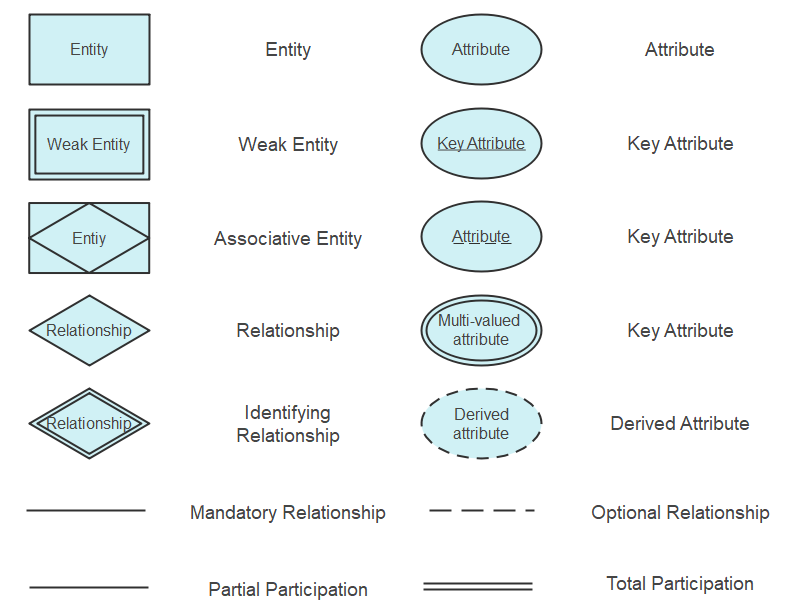
\includegraphics[width=0.4\linewidth]{images/chens-notation-1.png}
\end{figure}
\newpage
\section{The Relational Data Model}
\mydef{Set}{
A set is a well-defined collection of distinct objects, considered as an object in its own right. The objects in a set are called elements or members. Sets are usually denoted by capital letters like $A$, $B$, or $S$, and elements are listed within curly braces. For example, $A = \set{1, 2, 3}$ is a set containing the numbers 1, 2, and 3.
}

\mydef{Element of a Set}{
If $x$ is an element of set $A$, we write $x \in A$. If $x$ is not in $A$, we write $x \notin A$.
}

\mydef{Set-builder Notation}{
Set-builder notation is a shorthand used to describe a set by stating the properties that its elements must satisfy.
For example: $\set{x \in \mathbb{N} \mid x \text{ is even} }$ describes the set of even natural numbers.
}

\mydef{Cardinality}{
The cardinality of a set is the number of elements in the set, denoted $|A|$.
For example, if $A = \set{1, 2, 3}$, then $|A| = 3$.
}

\mydef{Cartesian Product} {
Let $A$ and $B$ be sets, then $A \times B = \set{(a,b) \mid a \in A , b \in B}$, e.g. $A=\{1,2\}, B=\{x,y\}, A \times B = \set{(1,x),(1,y),(2,x),(2,y)}$
}

\mydef{Subset}{
$A\subseteq B \Leftrightarrow \forall X. X\in A \Rightarrow X \in B$
}

\mydef{Proper Subset}{
$A \subset B \Leftrightarrow A\subseteq B \land A \neq B$
}

\mydef{Relation}{
$R \subseteq A \times B$. If $(a,b) \in R$, we say that $a$ is related to $b$ via $R$
}

\mydef{Left Total Relation}{
A relation $R \subseteq A \times B$ is left total (total on $A$) iff each element in $A$ is related to at least on element in $B$. $\forall a \in A.  \exists b \in B. (a,b) \in R$
}

\mydef{Right Unique Relation}{
A relation $R \subseteq A \times B$ is right unique iff each element in $A$ is related to at most one element in $B$. $\forall a\in A, \forall b1, b2 \in B, ((a,b1) \in R,(a,b2)\in R) \Rightarrow b1 = b2$
}

\mydef{Function}{
A function is left total and right unique relation. $f:A \to B$
}

\mydef{Partial Function}{
A partial function is a right unique relation, \textbf{not} necessarily left total. $f \rightharpoonup B$
}

\mydef{Set Union}{
$x \in A \cup B \Leftrightarrow x \in A \text{ or }  x \in B$
}

\mydef{Set Intersection}{
$x \in A \cap B \Leftrightarrow x \in A \text{ and } x \in B$
}

\mydef{Disjoint}{
We say two sets $A,B$ are disjoint iff $A \cap B=\phi$
}

\mydef{Relation Schema}{A declaration $\textstyle R\bigl(A_1{:}D_1,\dots,A_n{:}D_n\bigr)$ consisting of a name $R$, a finite, non‑empty attribute set $\set{A_i}$ and, for each attribute, its domain $\operatorname{dom}(A_i)=D_i$.}

\mydef{Schema Satisfaction}{A \emph{tuple} $t=(v_1,\dots,v_n)$ \emph{satisfies} the schema if $v_i\in D_i\;\forall i$.}

\mydef{Types}{\textit{Classes} of atomic values that share representation and operations, e.g. \texttt{Int}, \texttt{Real}, or \texttt{String}.}

\mydef{Domain}{A \textit{set} of atomic values with application‑specific semantics whose underlying implementation type is fixed.  Domains may define default values.  Example: $\textit{EmployeeAge}=\texttt{Int}[18,65]$.}

\commandnote{Domain declaration examples: \texttt{Name = String(20)}, \texttt{DollarPrice = Decimal(5,2)}.}



\mydef{Instance}{A \emph{finite set} of tuples that all satisfy a given relation schema.  While the schema is comparatively stable (static), its instance is \emph{dynamic}: it evolves through insertions, deletions, and updates.}

\minititle{Two Equivalent Views on Tuples}

\begin{itemize}
    \item \textbf{Positional (Cartesian‑product) view:} $t$ is an \emph{ordered list} $\bigl(v_1,\dots,v_n\bigr)$.  Column order carries meaning; attribute names are implicit.
    \item \textbf{Functional view:} Fix $A=\set{A_1,\dots,A_n}$ and $D=\bigcup_i D_i$.  Then a tuple is a \emph{function} $t:A\to D$ with $t(A_i)\in D_i$.  Here, order is irrelevant and attribute names are explicit.
\end{itemize}

\mydef{Domain Constraint}{Each attribute value must lie in its declared domain $D_i$.  Usually enforced by the DBMS type checker.}

\mydef{Functional Dependency (FD)}{For attribute sets $X,Y\subseteq A$, the notation $X\to Y$ states: for any two tuples $t_1,t_2$, equality of $X$‑values implies equality of $Y$‑values.  Written out: $t_1[X]=t_2[X]\Rightarrow t_1[Y]=t_2[Y]$.}

\mydef{Superkey}{An attribute set $K$ with $K\to A$ (it functionally determines the whole tuple).}

\mydef{Candidate Key}{A \emph{minimal} superkey — removing any attribute from it destroys the functional determination of $A$.}

\mydef{Primary Key}{The candidate key chosen by the database designer to serve as the principal identifier of tuples in a relation.  Remaining candidate keys are called \emph{alternate keys}.}

% -- revised example ------------------------------------------------------
\minititle{Example}
\begin{itemize}
    \item Relation schema $\textit{Employee}(\textit{EmpID},\textit{SSN},\textit{Email},\textit{Name},\textit{Dept})$.
    \item \emph{Superkeys} include any attribute set that uniquely identifies tuples, e.g $\{\textit{EmpID}\},\;\{\textit{SSN}\},\;\{\textit{EmpID},\textit{Name}\}$. The third set still determines the whole tuple but is \emph{not} minimal.
    \item \emph{Candidate keys}: the minimal superkeys $\{\textit{EmpID}\}\quad\text{and}\quad\{\textit{SSN}\}$. Each is irreducible.
    \item \emph{Primary key}: suppose we designate $\textit{EmpID}$ as the primary key.  The other candidate becomes an \emph{alternate key} available for unique look‑ups.
\end{itemize}

\mydef{Foreign Key}{Attribute(s) in relation $R$ whose values must also appear as the primary-key values of another relation $S$ (ensuring referential integrity).}

\commandnote{When an insertion, deletion or modification would break any constraint, the DBMS may (i) reject the change or (ii) repair it automatically (``cascade'', insert default/null, etc.).  The exact behaviour is part of the schema definition.}



\subsection*{A word on modeling different cardinalities}
Relational databases use foreign keys (FKs) to represent associations between entities. The modeling depends on the cardinality:

\minititle{One-to-One (1:1)}
A FK is placed in one of the tables.

\begin{center}
\begin{tabular}{|c|c|c|c|}
\hline
\textbf{Person} & ID (PK) & Name & PassportID (FK) \\
\hline
 & 1 & Alice & 101 \\
\hline
\end{tabular}
\quad
\begin{tabular}{|c|c|c|c|}
\hline
\textbf{Passport} & ID (PK) & Number & DateOfIssue \\
\hline
 & 101 & X1234 & 2020-01-01 \\
\hline
\end{tabular}
\end{center}

\minititle{One-to-Many (1:M) or Many-to-One (M:1)}
The FK is placed in the table on the "many" side, referencing the "one" side.

\begin{center}
\begin{tabular}{|c|c|c|}
\hline
\textbf{Department} & ID (PK) & Name \\
\hline
 & 1 & Human Resources \\
\hline
\end{tabular}
\quad
\begin{tabular}{|c|c|c|c|}
\hline
\textbf{Employee} & ID (PK) & Name & DepartmentID (FK) \\
\hline
 & 101 & John & 1 \\
\hline
\end{tabular}
\end{center}

\begin{center}
\end{center}

\minititle{Many-to-Many (M:M)}
Modeled via a relation table with two FKs, each referencing one of the related tables. The combination of FKs often serves as the primary key.

\begin{center}
    \begin{tabular}{|c|c|}
    \hline
    \textbf{StdID} & StdName \\
    \hline
    1 & Jane \\
    2 & Mark \\
    3 & Sara \\
    \hline
    \end{tabular}
    \quad
    \begin{tabular}{|c|c|}
    \hline
    \textbf{CourseID} & CourseTitle \\
    \hline
    10 & Database Systems \\
    11 & Operating Systems \\
    12 & Algorithms \\
    \hline
    \end{tabular}
    \quad
    \begin{tabular}{|c|c|}
    \hline
    \textbf{StdID} & \textbf{CourseID} \\
    \hline
    1 & 10 \\
    1 & 12 \\
    2 & 10 \\
    2 & 11 \\
    3 & 11 \\
    \hline
    \end{tabular}
    \end{center}

\newpage
\section{Functional Dependencies}
\mydef{Prime Attribute}{
An attribute that is part of any candidate key.
}

\mydef{Nonprime Attribute}{
An attribute that is not part of any candidate key.
}

\textbf{Example: }consider the simple relation \texttt{STUDENT(ID, Email, Name, Phone, CourseID)}. Possible super keys:
\[
\set{\texttt{ID}}, \set{\texttt{Email}}, \set{\texttt{ID}, \texttt{Name}}, \set{\texttt{ID}, \texttt{Email}, \texttt{Phone}}
\]
Only $\set{\texttt{ID}}$ and $\set{\texttt{Email}}$ are prime attributes.

\mydef{Trivial FD}{
We say that a functional dependency $X \to Y$ is \textbf{trivial} iff $Y \subseteq X$. 
}

\mydef{Full FD}{
A functional dependency $X \to Y$ is full iff for any $A \in X$, $(X-\set{A}) \to Y$ does not hold, i.e. you cannot remove any attribute from $X$ without breaking the dependency. Example: $\{$studentID, CourseID$\} \to $ Grade.
}

\mydef{Partial FD}{
A functional dependency $X \to Y$ is partial iff  $\exists A \in X$. $(X-\set{A}) \to Y$ holds.
}


\mydef{Transitive FD}{
A functional dependency $X \to Y$ is transitive in a relation $R$ iff $\exists \textbf{ Nonprime set of attributes } Z \in R$ and both $X \to Z$ and $Z \to Y$ hold.
}

\mydef{Inference}{
A functional dependency $X \to Y$ is \textbf{inferred} from a set of functional dependencies $F$ on a relation $R$ iff $X \to Y$ holds in every instance of $R$ that satisfies all dependencies in $F$
}

\minititle{Armstrong's Inference Rules for Functional Dependencies}
\begin{itemize}
    \item \textbf{IR1}: $(Y \subseteq X) \Rightarrow (X \to Y)$ (reflexive)
    \item \textbf{IR2}: $(X \to Y) \Rightarrow (X \cup Z \to Y \cup Z)$ (augmentation) 
    \item \textbf{IR3}: $((X \to Y) \land (Y \to Z)) \Rightarrow X \to Z$ (transitive) 
\end{itemize}

\mydef{Closure}{
The closure of attribute set $X$ under a set of functional dependencies $F$, denoted as $X_F^+$ is the set of all attributes that $X$ can determine using FDs in $F$. $X_F^+ = \set{A \mid X \to A \in F \text{ or can be inferred from it}}$ 
}

\minititle{Closure Algorithm}
\begin{itemize}
    \item input: a set $F$ of FDs on a relation $R$, and a set of attributes $X$ contained in $R$
    \item initialization: $X_F^+ = X$
    \item changed = True
    \item while changed:
    \begin{enumerate}
        \item changed = False
        \item for each FD $Y \to Z \in F$:
        \begin{enumerate}
            \item If $(Y \subseteq X_F^+) \land (Z \notin X_F^+)$:
            \begin{enumerate}
                \item $X_F^+ = X_F^+ \cup \set{Z}$
                \item changed = True
            \end{enumerate}
        \end{enumerate}
    \end{enumerate}
    \item Output: $X_F^+$
\end{itemize}

\mydef{FDs Verification}{
$F \text{ implies }X \to Y \textit{ iff } Y \subseteq X_F^+$
}

\mydef{Superkeys Verification}{
$X$ is a super key for $R$ with attribute set $U$ \textit{iff} $X_F^+ = U$
}
\newpage
\minititle{Finding Candidate Keys}
\begin{verbatim}
Input: Relation (R) over set of attributes (U), set of FDs (F)
initialization: K:= U
minimal = False
while not minimal
    minimal = True
    for each attribute A in K
        compute closure of (K-A) under F
            if the closure = U
                set K := K - {A}
                minimal = False
Return: K
\end{verbatim}

\mydef{Coverage}{
For any two sets of functional dependencies $F_1, F_2$, we say that $F_1$ covers $F_2$, \textit{iff}  $\forall X \to Y \in F_2. Y \subseteq X_{F_1}^+$.   
}


\mydef{Equivalence}{
For any two sets of functional dependencies $F_1, F_2$, we say they are equivalent, \textit{iff} they cover each other.   
}
Example: verify whether the following FDs are equivalent.
\begin{itemize}
    \item $F_1=\set{A \to C, AC \to D, E \to AD, E \to H}$ and
    \item $F_2 = \set{A \to CD, E \to AH}$
\end{itemize}
We check first if $F_1$ covers $F_2$
\begin{itemize}
    \item considering $A \to \set{C,D} \quad \set{C,D} \in A_{F_1}^+ = \set{A,C,D}$
    \item considering $E \to \set{A,H} \quad \set{A,H} \in E_{F_1}^+ = \set{E,A,D,H,C}$
    \item Hence $F_1$ covers $F_2$
\end{itemize}

Next, we check first if $F_2$ covers $F_1$
\begin{itemize}
    \item considering $A \to C \quad C \in A_{F_2}^+ = \set{C,D}$
    \item considering $\set{A,C} \to D \quad D \in \set{A,C}_{F_2}^+ = \set{A,C,D}$
    \item considering $E \to \set{A,D} \quad \set{A,D} \in E_{F_2}^+ = \set{A,H,C,D}$
    \item considering $E \to H \quad H \in E_{F_2}^+ = \set{A,H,C,D}$
    \item Hence $F_2$ covers $F_1$
\end{itemize}

Therefore, they are equivalent

\mydef{Redundancy}{
A functional dependency $f = X \to A$ is redundant in FDs set $F$ \textit{iff} $A \subseteq X_G^+$ where $G = F-\set{X \to A}$, i.e. $F - \set{f}$ implies $f$. 
}

\mydef{Extraneous}{
Given a set $F$ of FDs and one $f=AX \to B \in F$, then $A$ is extraneous if $B \subseteq X_F^+$
}


\mydef{Minimal cover}{
A set of FDs $F$ is a minimal cover of a set of FDs $E$ iff $F$ covers $E$ and there is no $f \in F. \quad F- \set{f}$ covers $E$
}

\mydef{Canonical}{
    A functional dependency $f=X \to Y$ is in a canonical form iff $|Y|=1$
}

\mydef{Minimal set of FDs}{
A set $F$ of FDs is minimal iff it satisfies the following conditions: (i) All FDs in a canonical form. (ii) No extraneous attributes. (iii) No redundant FDs.
}

\minititle{Steps to Obtain a Minimal Set of Functional Dependencies}
\begin{enumerate}
    \item Transform to Canonical form
    \item Remove Extraneous Attributes
    \item Remove Redundant FDs
\end{enumerate}

\newpage
\section{Relational Algebra and SQL}
\mydef{Data Model}{
    In relational databases, the data model specifies how data is structured and how it can be manipulated. i.e. it says that data is organized into tables (called relations) with columns (attributes) and rows (tuples).
}

\mydef{Relational model}{
    In relational databases, the relational model represent data as relations (tables). Each relation has constraints, such as keys or data types, to ensure data integrity.
}

\mydef{Relational Algebra}{
    The formal system for manipulating relations. It provides a theoretical foundation for \textbf{Query} operations used in relational databases
}

\mydef{Algebra}{
    A formal system in which expressions are constructed using operators and atomic operands. These expressions can be evaluated, and two expressions are considered equivalent if they yield the same result for all possible values of their operands.
}

\mydef{Relational Algebra}{
    A type of algebra where the operands are relations (tables), and the operators are defined for any instance of those relations. Operations can be combined to form complex expressions, and evaluating an expression produces a result schema (the structure of the output) and a result instance (the actual data produced).
}

\mydef{SQL}{
    The Standard Query Language (SQL) is the language used to interact with relational databases. It is a \textbf{declarative} language, meaning that when you write a query, you describe what result you want, not how the database should compute it. This contrasts with procedural languages, where you must specify every step.
}

\minititle{SQL Structure}
SQL is organized into several sub-languages, each serving a distinct purpose:
\begin{itemize}
    \item Data Definition Language (DDL): used to define or alter the structure of database objects. Commands used such as: \texttt{CREATE, ALTER, DROP}
    \item Data Manipulation Language (DML): used to retrieve and manipulate data. Command used such as: \texttt{SELECT, UPDATE, INSERT, DELETE}
    \item Data Control Language (DCL): manages user permissions and access control. Commands used such as: \texttt{GRANT, REVOKE}
    \item Transaction Control Language (TCL): manages database transactions. Commands used such as: \texttt{COMMIT ROLLBACK}
\end{itemize}

Example DML Queries:
\begin{verbatim}
    SELECT name, age FROM Student WHERE age >= 18 ORDER BY name ASC;
    
    INSERT INTO Student (stdId, name, age) VALUES (101, "Alice", 20);
    
    UPDATE Student SET age = age + 1 WHERE stdId = 101;

    DELETE FROM Student WHERE stdId = 101;
\end{verbatim}

Examples on \texttt{COUNT, DISTINCT, EXIST, IN}
\begin{verbatim}
    SELECT COUNT(*) FROM Student;

    SELECT COUNT(DISTINCT stdID) FROM Student; 
    
    SELECT * FROM employees e
    WHERE EXISTS (
        SELECT 1
        FROM bonus b
        WHERE b.employee_id = e.employee_id
    );

    SELECT * FROM employees WHERE department_id IN (1, 2, 5);

\end{verbatim}

\newpage
Example DDL Queries:
\begin{verbatim}
    CREATE TABLE Course (courceID INT PRIMARY KEY,
                         title    VARCHAR(100)
                        );

    ALTER TABLE Course ADD COLUMN credits INT;

    DROP TABLE Course;
\end{verbatim}

Example DCL Queries:
\begin{verbatim}
    GRANT SELECT, INSERT ON Student TO user1;

    REVOKE INSERT ON Student FROM user1;
\end{verbatim}

Example TCL Queries:
\begin{verbatim}
    BEGIN;
    UPDATE Account SET balance = balance - 100 WHERE id = 1;
    COMMIT; 
\end{verbatim}
Example Primary Key and Foreign Key:
\begin{verbatim}
CREATE TABLE Department (
    deptID INT PRIMARY KEY,
    deptName VARCHAR(100)
);

CREATE TABLE Employee (
    empID INT PRIMARY KEY,
    empName VARCHAR(100),
    deptID INT,
    FOREIGN KEY (deptID) REFERENCES Department(deptID)
);
\end{verbatim}

Example Composite Primary Key:
\begin{verbatim}
    CREATE TABLE Student (
    stdID INT PRIMARY KEY,
    stdName VARCHAR(100)
);

CREATE TABLE Course (
    crsID INT PRIMARY KEY,
    crsName VARCHAR(100)
);

CREATE TABLE Enrollment (
    stdID INT,
    crsID INT,
    grade CHAR(2),
    PRIMARY KEY (stdID, crsID),
    FOREIGN KEY (stdID) REFERENCES Student(stdID),
    FOREIGN KEY (crsID) REFERENCES Course(crsID)
);
\end{verbatim}

Example Domain Constraints:
\begin{verbatim}
CREATE TABLE Product (
    id INT PRIMARY KEY,
    price DECIMAL(10,2) CHECK (price >= 0),
    category VARCHAR(50) NOT NULL
);
\end{verbatim}

\minititle{Set Operators}
\mydef{Arity / Degree}{
let $R(A_1, \cdots, A_n)$ be a relation schema, the arity of $R$ is $\text{arity}(R)=n$
}

\mydef{Union Compatible}{
   We say that relations $R(A_1, \cdots, A_n)$ and $S(B_1, \cdots, B_n)$ are union compatible if $\text{artiy}(R) = \text{arity}(S)$ and $ \text{dom}(A_i)=\text{dom}(B_i) \quad \forall i \in \{1, \cdots, n\}$
}

\mydef{Relation Union}{$R_1 \cup R_2 = \set{t \mid t \in R_1 \lor t \in R_2}$. SQL Equiv.: \texttt{SELECT * FROM R UNION SELECT * FROM S}}



\mydef{Relation Intersection}{$R_1 \cap R_2 = \set{t \mid t \in R_1 \land t \in R_2}$. SQL: \texttt{SELECT * FROM R INTERSECT SELECT * FROM S}}

\mydef{Relation Difference}{$R_1 - R_2 = \set{t \mid t \in R_1 \land  t \notin R_2}$. SQL: \texttt{SELECT * FROM R EXCEPT SELECT * FROM S}}

\mydef{Relation Cartesian Product}{
$R_1 \times R_2 = \set{t_1 \circ t_2 \mid t_1 \in R_1,\ t_2 \in R_2}$. SQL: \texttt{SELECT * FROM R CROSS JOIN S}}

\minititle{Relation Operators (Unary)}
\mydef{Rename}{
    Changes the schema of the relation $R$ by renaming attribute $A_1$ to $B_1$ and so on. $\rho_{(B1, \cdots, B_n \leftarrow A_1, \cdots, A_n)}(R)$. SQL: \texttt{SELECT a AS b FROM R AS R1}
}

\mydef{Selection}{
  $\sigma_C(R) = \set{t \in R \mid C(t)}$ is the set of all tuples in $R$ that satisfy the condition $C$.\\
  The condition $C$ is a Boolean expression composed of predicates:
  \[
  C = P_1\ \mathit{op}_1\ P_2\ \mathit{op}_2\ \cdots\ \mathit{op}_{n-1}\ P_n
  \]
  where each operator $\mathit{op}_i \in \{\text{AND},\ \text{OR},\ \text{NOT}\}$, and each predicate $P_i$ has the form:
  \[
  P_i ::= A\ \theta\ B \quad \text{or} \quad A\ \theta\ c
  \]
  with attributes $A$, $B$, constant $c$, and comparison operator $\theta \in \{=,\ <,\ \leq,\ >,\ \geq,\ \neq\}$.
}

SQL Equiv. : \texttt{SELECT * FROM R WHERE C}

\mydef{Projection}{
    $\Pi_Y(R) = \set{t[Y] \mid t \in R}$. SQL: \texttt{SELECT Y FROM R}
}

\mydef{Idempotent}{
  An operator $\mathcal{O}$ is called \emph{idempotent} if applying it multiple times has the same effect as applying it once: $\mathcal{O}(\mathcal{O}(x)) = \mathcal{O}(x) \quad \forall x$. \textbf{Projection} is \textit{Idempotent}
}


\minititle{Relation Operators (Binary)}
\mydef{Theta Join}{
    $R_1 \Join_C R_2 = \set{t_1 \circ t_2 \mid t_1 \in R_1 \land t_2 \in R_2 \land C(t_1 \circ t_2)} = \sigma_C(R_1 \times R_2)$
}

\textbf{Example:} \texttt{SELECT * FROM Employee JOIN Bonus ON Employee.salary > Bonus.threshold}
\[
\begin{array}{ccc}
\begin{tabular}{|c|c|}
\hline
id & salary \\
\hline
1 & 50000 \\
2 & 30000 \\
\hline
\end{tabular}
&
\begin{tabular}{|c|}
\hline
threshold \\
\hline
20000 \\
40000 \\
\hline
\end{tabular}
&
\begin{tabular}{|c|c|c|}
\hline
id & salary & threshold \\
\hline
1 & 50000 & 20000 \\
1 & 50000 & 40000 \\
2 & 30000 & 20000 \\
\hline
\end{tabular}
\end{array}
\]

\mydef{Equi-Join}{
    Theta Join with $C$ consists only of equality comparison.
}

\textbf{Example:} \texttt{SELECT * FROM Orders JOIN Customers ON Orders.cust\_id = Customers.id}

\[
\begin{array}{ccc}
\begin{tabular}{|c|c|}
\hline
order\_id & cust\_id \\
\hline
101 & 1 \\
102 & 2 \\
103 & 4 \\
\hline
\end{tabular}
&
\begin{tabular}{|c|c|}
\hline
id & name \\
\hline
1 & Alice \\
2 & Bob \\
3 & Carol \\
\hline
\end{tabular}
&
\begin{tabular}{|c|c|c|c|}
\hline
order\_id & cust\_id & id & name \\
\hline
101 & 1 & 1 & Alice \\
102 & 2 & 2 & Bob \\
\hline
\end{tabular}
\end{array}
\]

\mydef{Natural Join}{
    Equi-Join where $C$ is quality on common attributes and duplicate common attributes are removed from the result.
}

\textbf{Example: }\texttt{SELECT * FROM Employee NATURAL JOIN Department}
\[
\begin{array}{ccc}
\begin{tabular}{|c|c|}
\hline
emp\_id & dept\_id \\
\hline
1 & 10 \\
2 & 20 \\
3 & 10 \\
4 & 40 \\
5 & 50 \\
\hline
\end{tabular}
&
\begin{tabular}{|c|c|}
\hline
dept\_id & name \\
\hline
10 & HR \\
20 & IT \\
30 & Sales \\
60 & Legal \\
\hline
\end{tabular}
&
\begin{tabular}{|c|c|c|}
\hline
emp\_id & dept\_id & name \\
\hline
1 & 10 & HR \\
2 & 20 & IT \\
3 & 10 & HR \\
\hline
\end{tabular}
\end{array}
\]

\mydef{Outer Join}{
    Natural Join but preserves unmatched tuples by padding them with NULL values. That can be done on the relation on the left, right or both.
}

\mydef{Left Outer Join}{
    Includes all tuples from the left relation, padding unmatched right-side tuples with NULLS.
}

\textbf{Example: }\texttt{SELECT * FROM Orders LEFT OUTER JOIN Customers ON Orders.cust\_id = Customers.id}
\[
\begin{array}{ccc}
\begin{tabular}{|c|c|}
\hline
order\_id & cust\_id \\
\hline
101 & 1 \\
102 & 2 \\
103 & 4 \\
\hline
\end{tabular}
&
\begin{tabular}{|c|c|}
\hline
id & name \\
\hline
1 & Alice \\
2 & Bob \\
3 & Carol \\
\hline
\end{tabular}
&
\begin{tabular}{|c|c|c|c|}
\hline
order\_id & cust\_id & id & name \\
\hline
101 & 1 & 1 & Alice \\
102 & 2 & 2 & Bob \\
103 & 4 & \text{NULL} & \text{NULL} \\
\hline
\end{tabular}
\end{array}
\]

\mydef{Right Outer Join}{
    Includes all tuples from the right relation, padding unmatched left-side tuples with NULLS.
}

\textbf{Example: }\texttt{SELECT * FROM Orders RIGHT OUTER JOIN Customers ON Orders.cust\_id = Customers.id}
\[
\begin{array}{ccc}
\begin{tabular}{|c|c|}
\hline
order\_id & cust\_id \\
\hline
101 & 1 \\
102 & 2 \\
103 & 4 \\
\hline
\end{tabular}
&
\begin{tabular}{|c|c|}
\hline
id & name \\
\hline
1 & Alice \\
2 & Bob \\
3 & Carol \\
\hline
\end{tabular}
&
\begin{tabular}{|c|c|c|c|}
\hline
order\_id & cust\_id & id & name \\
\hline
101 & 1 & 1 & Alice \\
102 & 2 & 2 & Bob \\
\text{NULL} & \text{NULL} & 3 & Carol \\
\hline
\end{tabular}
\end{array}
\]

\mydef{Full Outer Join}{
    Includes all tuples from both relations, padding unmatched tuples from either side with NULLS.
}
\textbf{Example: }\texttt{SELECT * FROM Orders FULL OUTER JOIN Customers ON Orders.cust\_id = Customers.id}
\[
\begin{array}{ccc}
\begin{tabular}{|c|c|}
\hline
order\_id & cust\_id \\
\hline
101 & 1 \\
102 & 2 \\
103 & 4 \\
\hline
\end{tabular}
&
\begin{tabular}{|c|c|}
\hline
id & name \\
\hline
1 & Alice \\
2 & Bob \\
3 & Carol \\
\hline
\end{tabular}
&
\begin{tabular}{|c|c|c|c|}
\hline
order\_id & cust\_id & id & name \\
\hline
101 & 1 & 1 & Alice \\
102 & 2 & 2 & Bob \\
103 & 4 & \text{NULL} & \text{NULL} \\
\text{NULL} & \text{NULL} & 3 & Carol \\
\hline
\end{tabular}
\end{array}
\]

\minititle{Operators Properties}
\begin{table}[h]
\centering
\begin{tabular}{|l|l|l|c|c|c|c|}
\hline
\textbf{Operator} & \textbf{Result Schema} & \textbf{Result Size} & \textbf{Comm.} & \textbf{Assoc.} & \textbf{Idem.} & \textbf{Duplicates} \\
\hline
Union & Same as inputs & $\leq |R| + |S|$ & Yes & Yes & No & No \\
\hline
Intersection & Same as inputs & $\leq \min(|R|, |S|)$ & Yes & Yes & Yes & No \\
\hline
Difference & Same as $R$ & $\leq |R|$ & No & No & No & No \\
\hline
Cartesian Product & $R \cup S$ & $|R| \cdot |S|$ & Yes & Yes & No & Yes \\
\hline
Rename & Same & $|R|$ & N/A & N/A & N/A & N/A \\
\hline
Selection & Same as $R$ & $\leq |R|$ & Yes & Yes & No & Yes \\
\hline
Projection & Subset of $R$ & $\leq |R|$ & No & No & Yes & No \\
\hline
Theta Join & $R \cup S$ & $[0,\ |R| \cdot |S|]$ & No & No & No & Yes \\
\hline
Equi-Join     & $R \cup S$ & $[0,\ |R| \cdot |S|]$ & No & No & No & Yes \\
\hline
Natural Join & $R \cup S\setminus C$ & $[0,\ |R| \cdot |S|]$ & Yes & Yes & No & Yes \\
\hline
Left Outer Join & $R \cup S$ & $\geq |R|$ & No & No & No & Yes \\
\hline
Right Outer Join & $R \cup S$ & $\geq |S|$ & No & No & No & Yes \\
\hline
Full Outer Join & $R \cup S$ & $\geq \max(|R|, |S|)$ & No & No & No & Yes \\
\hline
\end{tabular}
\end{table}


\minititle{Common Datatypes}
\begin{table}[h]
\centering
\begin{tabular}{|l|l|}
\hline
\textbf{Category} & \textbf{Common Data Types} \\ \hline
Numeric           & INT, BIGINT, DECIMAL(p,s), FLOAT, DOUBLE \\ \hline
Character         & CHAR(n), VARCHAR(n), TEXT                 \\ \hline
Date/Time         & DATE, TIME, TIMESTAMP, DATETIME           \\ \hline
Boolean           & BOOLEAN / BOOL                             \\ \hline
\end{tabular}
\end{table}

\newpage
\minititle{Algebra to SQL Example}
\[
\pi_{\text{supplier\_name},\ \text{product\_name}} \left(
  \sigma_{\text{price} > 50} \left(
    \left(
      \text{Suppliers} \bowtie_{\text{supplier\_id}} \text{Products}
    \right)
    \bowtie_{\text{category\_id}} \text{Categories}
  \right)
\right)
\]

\begin{verbatim}
WITH SupplierProducts AS (
    SELECT 
        s.supplier_name, 
        p.product_name, 
        p.price, 
        p.category_id
    FROM Suppliers s
    JOIN Products p ON s.supplier_id = p.supplier_id
),
Filtered AS (
    SELECT * FROM SupplierProducts WHERE price > 50
)
SELECT f.supplier_name, f.product_name
FROM Filtered f
JOIN Categories c ON f.category_id = c.category_id;
\end{verbatim}

\newpage
\section{Normal Forms}
\mydef{Normalization}{
    Decomposing a large schema $R(A)$ into smaller schemata $R_i(A_i)$ with $A_i \subset A$ to minimize redundancy, avoid information loss and preserve functional dependencies.
}

\mydef{Spurious Tuples}{
   Decomposing a relation into multiple relations as part of normalization can lead to spurious tuples when these relations are rejoined (tuples that did not exist in the original relation).
}
\textbf{Example}
\begin{figure}[H]
    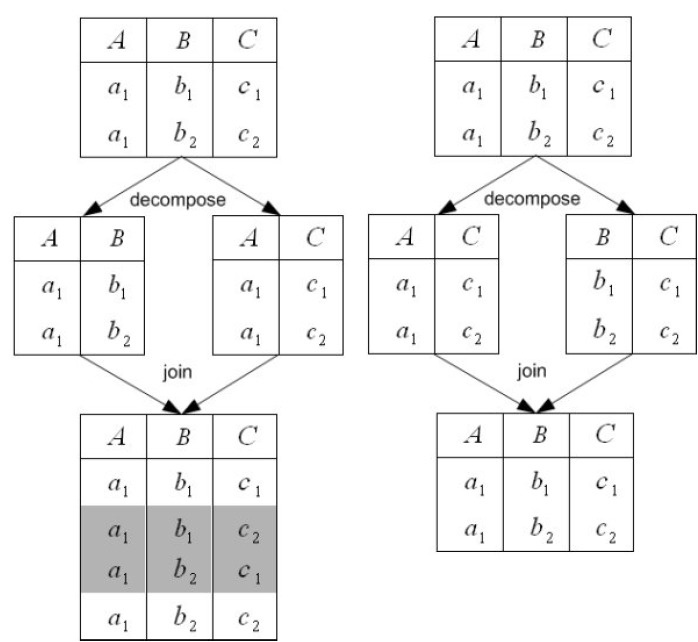
\includegraphics[width=0.3\linewidth]{images/supurious.png}
\end{figure}

\mydef{Lossless-Join Decomposition}{
    We call a decomposition of $R(A,B,C)$ into $R_1(A,B)$ and $R_2(B,C)$ lossless-join iff, for all instances $r$ of $R$ that respect the FDs, the following identity holds: $r = \Pi_{A,B}(r) \Join \Pi_{B,C}(r)$
}

\textbf{Example (Lossless): }Consider the relation: \texttt{empDept(empID, name, deptID, deptName)} with FDs: 
\begin{align*}
\texttt{empID} &\to \texttt{name} \\
\texttt{empID} &\to \texttt{deptID} \\
\texttt{deptID} &\to \texttt{deptName}
\end{align*}

We decompose the relation into:
\begin{itemize}
  \item \texttt{emp(empID, name, deptID)}
  \item \texttt{dept(deptID, deptName)}
\end{itemize}
Consider legal instances $r$:
\begin{tabular}{cccc}
\toprule
\textbf{empID} & \textbf{name} & \textbf{deptID} & \textbf{deptName} \\
\midrule
1 & Alice & 10 & CS \\
2 & Bob & 10 & CS \\
3 & Carol & 20 & Math \\
\bottomrule
\end{tabular}

$\Pi_{\text{empID, name, deptID}}(r)$
\begin{tabular}{ccc}
\toprule
\textbf{empID} & \textbf{name} & \textbf{deptID} \\
\midrule
1 & Alice & 10 \\
2 & Bob & 10 \\
3 & Carol & 20 \\
\bottomrule
\end{tabular}

$\Pi_{\text{deptID, deptName}}(r)$
\begin{tabular}{cc}
\toprule
\textbf{deptID} & \textbf{deptName} \\
\midrule
10 & CS \\
20 & Math \\
\bottomrule
\end{tabular}

$\Pi_{\text{deptID, deptName}}(r) \Join \Pi_{\text{deptID, deptName}}(r)$
\begin{tabular}{cccc}
\toprule
\textbf{empID} & \textbf{name} & \textbf{deptID} & \textbf{deptName} \\
\midrule
1 & Alice & 10 & CS \\
2 & Bob & 10 & CS \\
3 & Carol & 20 & Math \\
\bottomrule
\end{tabular}
$=r$

\textbf{Example (Lossy): }Consider the relation: \texttt{R(empName, empLevel, empSalary)} with FDs: 
\begin{align*}
\texttt{empName} &\to \texttt{empLevel} \\
\texttt{empName} &\to \texttt{empSalary} \\
\texttt{empLevel} &\to \texttt{empSalary}
\end{align*}

Consider legal instances $r$:
\begin{tabular}{ccc}
\toprule
\textbf{empName} & \textbf{empLevel} & \textbf{empSalary} \\
\midrule
Alice & Junior & 50K \\
Bob   & Junior & 50K \\
Carol & Senior & 50K \\
\bottomrule
\end{tabular}

$\Pi_{\text{empName, empSalary}}(r)$
\begin{tabular}{cc}
\toprule
\textbf{empName} & \textbf{empSalary} \\
\midrule
Alice & 50K \\
Bob   & 50K \\
Carol & 50K \\
\bottomrule
\end{tabular}

$\Pi_{\text{empLevel, empSalary}}(r)$
\begin{tabular}{cc}
\toprule
\textbf{Level} & \textbf{Salary} \\
\midrule
Junior & 50K \\
Senior & 50K \\
\bottomrule
\end{tabular}

$\Pi_{\text{empName, empSalary}}(r) \Join \Pi_{\text{empLevel, empSalary}}(r)$

\begin{tabular}{ccc}
\toprule
\textbf{empName} & \textbf{empLevel} & \textbf{empSalary} \\
\midrule
Alice & Junior & 50K \\
Alice & Senior & 50K \\
Bob   & Junior & 50K \\
Bob   & Senior & 50K \\
Carol & Junior & 50K \\
Carol & Senior & 50K \\
\bottomrule
\end{tabular}
$\neq r$

\commandnote{
    A decomposition of $R(A,B,C)$ into $R_1(A,B)$ and $R_2(B,C)$ is lossless-join iff $B$ is a \textbf{superkey} in $R_1$ \textit{or} $R_2$
}

\mydef{Dependency-Preserving}{
    We call a decomposition dependency preserving if the \textit{union} of FDs from decomposed relations yields all FDs in the original relation.
}

\textbf{Example: }If we decompose \texttt{R(empName, empLevel, empSalary)} into \texttt{R1(empName, empLevel), R2(empName, empSalary)}. This is a \textbf{lossless-join} decomposition:

$\Pi_{\text{empName, empLevel}}(r)$
\begin{tabular}{cc}
\toprule
\textbf{empName} & \textbf{empLevel} \\
\midrule
Alice & Junior \\
Bob   & Junior \\
Carol & Senior \\
\bottomrule
\end{tabular}

$\Pi_{\text{empName, empSalary}}(r)$
\begin{tabular}{cc}
\toprule
\textbf{empName} & \textbf{Salary} \\
\midrule
Alice & 50K \\
Bob   & 50K \\
Carol & 50K \\
\bottomrule
\end{tabular}

$\Pi_{\text{empName, empLevel}}(r) \Join \Pi_{\text{empName, empSalary}}(r)$

\begin{tabular}{ccc}
\toprule
\textbf{empName} & \textbf{empLevel} & \textbf{empSalary} \\
\midrule
Alice & Junior & 50K \\
Bob   & Junior & 50K \\
Carol & Senior & 50K \\
\bottomrule
\end{tabular}
$=r$

\textbf{However, }This is not \textit{dependency preserving}. Proof:

FDs of $R_1 = \set{\texttt{empName} \to \texttt{empLevel}}$

FDs of $R_2 = \set{\texttt{empName} \to \texttt{empSalary}} $

The union of both is $\set{\texttt{empName} \to \texttt{empLevel}, \texttt{empName} \to \texttt{empSalary}}$ which is not equal to $\set{\texttt{empName} \to \texttt{empLevel},
\texttt{empName} \to \texttt{empSalary},
\texttt{empLevel} \to \texttt{empSalary}}$
i.e. the FD $\texttt{empLevel} \to \texttt{empSalary}$ is \textbf{lost}!

\textbf{Example (Lossless-join and Dependency Preserving Decomposition)}

$R_1(empName, empLevel), R_2(empLevel, empSalary)$
\begin{itemize}
    \item Lossless-join becasue \texttt{empLevel} is superkey in $R_2$
    \item Dependency Preserving becasue $F_1 \cup F_2 = \set{{empName} \to \texttt{empLevel}, \texttt{empLevel} \to \texttt{empSalary}}$ and \textit{through transitivity} we get $\set{{empName} \to \texttt{empSalary}}$
\end{itemize}

\minititle{The Chase Test to Check the Lossless-Join Property}
\textbf{Input:}
\begin{itemize}
    \item A relation schema \( R = \{A_1, A_2, \dots, A_n\} \)
    \item A set of functional dependencies \( F \)
    \item A decomposition \( \mathcal{D} = \{R_1, R_2, \dots, R_k\} \)
\end{itemize}

\textbf{Goal:} Determine whether the decomposition is \textbf{lossless-join} with respect to \( F \).

\bigskip

\textbf{Procedure:}
\begin{enumerate}[label=\textbf{Step \arabic*.}, leftmargin=2.5em]
    \item \textbf{Initialize a Chase Table:}
    \begin{itemize}
        \item Create a table with one row per sub-relation \( R_i \in \mathcal{D} \), and one column per attribute \( A_j \in R \).
        \item For each row \( i \) and attribute \( A_j \):
        \begin{itemize}
            \item If \( A_j \in R_i \), set the cell to \( \alpha_{A_j} \)
            \item If \( A_j \notin R_i \), set the cell to a unique symbol \( \beta_{iA_j} \)
        \end{itemize}
    \end{itemize}
    
    \item \textbf{Apply Functional Dependencies:}
    \begin{itemize}
        \item For each FD \( X \to Y \in F \), and for each row:
        \begin{itemize}
            \item If all attributes in \( X \) have the same symbol in the row (e.g., all equal to \( \sigma \)),
            \item Then set each attribute in \( Y \) to that same symbol \( \sigma \)
        \end{itemize}
        \item Repeat until no further changes occur in the table.
    \end{itemize}
    
    \item \textbf{Check for Losslessness:}
    \begin{itemize}
        \item If any row contains only the original \( \alpha_{A_j} \) symbols across all attributes, the decomposition is \textbf{lossless}.
        \item Otherwise, it is \textbf{lossy}.
    \end{itemize}
\end{enumerate}

\minititle{Example (Lossless)}

Let \( R(A, B, C) \), with FDs \( F = \{ A \to B \} \), and decomposition:
\[
R_1(A, B), \quad R_2(A, C)
\]

\textbf{Initial Chase Table:}

\begin{tabular}{ccc}
\toprule
A & B & C \\
\midrule
\( \alpha_A \) & \( \alpha_B \) & \( \beta_{1C} \) \\
\( \alpha_A \) & \( \beta_{2B} \) & \( \alpha_C \) \\
\bottomrule
\end{tabular}

\textbf{Apply } \( A \to B \):  
\begin{tabular}{ccc}
\toprule
A & B & C \\
\midrule
\( \alpha_A \) & \( \alpha_B \) & \( \beta_{1C} \) \\
\( \alpha_A \) & \( \alpha_B \) & \( \alpha_C \) \\
\bottomrule
\end{tabular}

Since row 2 contains only \(\alpha\)-symbols, the decomposition is \textbf{lossless}.

\minititle{Example (Lossy)}

Let \( R(A, B, C) \), with FDs \( F = \{ A \to B \} \), and decomposition:
\[
R_1(A, B), \quad R_2(B, C)
\]

\textbf{Initial Chase Table:}

\begin{tabular}{ccc}
\toprule
A & B & C \\
\midrule
\( \alpha_A \) & \( \alpha_B \) & \( \beta_{1C} \) \\
\( \beta_{2A} \) & \( \alpha_B \) & \( \alpha_C \) \\
\bottomrule
\end{tabular}

\textbf{Apply } \( A \to B \):  
Only row 1 has \( A = \alpha_A \), but \( B = \alpha_B \) already → no changes.

No row becomes all-\(\alpha\), so the decomposition is \textbf{lossy}.

\mydef{1NF}{
    A relation is in First Normal Form (1NF) iff the domain contains only atmoic single values.
}

\minititle{2NF}
A relation is in Second Normal Form iff:
\begin{itemize}
    \item It is in 1NF
    \item There is no \textit{non-prime} attribute $A$ such that $Y \to A \in F$, where $Y$ is a proper subset of a candidate key $K$ ($Y \subsetneq K$)
\end{itemize}
In other words, if all \textit{candidate} keys consist of a single attribute, 2NF is guaranteed.

\textbf{Example: }Consider the relation \texttt{EMP\_PROJ}(\texttt{EmpID, EmpName, ProjId, ProjName, ProjLocation, Hours}) With Candidate Key \texttt{(EmpID, ProjId)} and set of FDs:\\
$\set{
    (\texttt{EmpID, ProjId} \to \texttt{Hours}),\\
    (\texttt{EmpID} \to \texttt{EmpName}),\\
    (\texttt{ProjId} \to \texttt{ProjName, ProjLocation})
}$

\texttt{EmpName} is a \textit{non-prime} attribute that is determined by \texttt{EmpID} $\subsetneq \set{\texttt{EmpID, ProjId}}$ Hence 2NF is violated. (the same applies for \texttt{ProjName, ProjLocation})

\textbf{Normalization}
This relation can be normalized to 2NF by decomposing it in a way so we do not have these \textit{partial} dependencies on the primary key:
\texttt{EMP(EmpID, EmpName)}, \texttt{PROJ(ProjID, ProjName, ProjLocation)}, \texttt{EMP\_PROJ(EmpID, ProjID, Hours)}

\minititle{3NF}
A relation is in Third Normal Form iff it is in 2NF and for each FD $X \to Y$, one of the following statements holds:
\begin{itemize}
    \item $X \to Y$ is trivial ($Y \subseteq X$)
    \item $X$ is a \textbf{superkey}
    \item Every attribute $A \in Y - X$ is a \textit{prime} attribute
\end{itemize}

\textbf{Example: }Consider the relation \texttt{EMP\_DEPT(}%
\texttt{EmpID}, %
\texttt{EmpName}, %
\texttt{EmpBD}, %
\texttt{EmpAddress}, %
\texttt{DeptID}, %
\texttt{DeptName}, %
\texttt{DeptMgrId}%
\texttt{)}
With FDs:
\begin{itemize}
    \item \texttt{EmpID} $\to$ \texttt{EmpName}, \texttt{EmpAddress}, \texttt{EmpBD}, \texttt{DeptID}
    \item \texttt{DeptID} $\to$ \texttt{DeptName}, \texttt{DeptMgrId}
\end{itemize}

For FD1, \texttt{EmpID} is superkey (we are safe). For FD2 it is not trivial, \texttt{DeptID} is not superkey, and none of \texttt{DeptName} or \texttt{DeptMgrId} is prime. So this violates 3NF.

\minititle{Normalization}
We must remove transitive dependencies to normalize to 3NF.
\begin{itemize}
    \item \texttt{EMP(}%
\texttt{EmpID}, %
\texttt{EmpName}, %
\texttt{EmpBD}, %
\texttt{EmpAddress}, %
\texttt{DeptID}
\texttt{)}
    \item \texttt{DEPT(}%
\texttt{DeptID}, %
\texttt{DeptName}, %
\texttt{DeptMgrId}%
\texttt{)}
\end{itemize}

\minititle{BCNF}
A relation $R$ is Boyce-Codd Normal Form (BCNF) iff for each FD $X \to Y$, one the following statements holds:
\begin{itemize}
    \item $Y \subseteq X$ (trivial)
    \item $X$ is a \textit{superkey}
\end{itemize}

\textbf{Note: }Relations that violate BCNF are rare and hard to find in practice. In real projects, normalizing to 3NF usually guarantee BCNF except for some rare cases.

\textbf{Example: }Assume we are building a system to manage land properties across different districts. Each property is assigned a globally unique property ID.

Locally, properties are identified by the lot number, which is only unique within a district. A property is uniquely identified by district and lot number.

Additionally, each property belongs to one area (each district has multiple areas)

Condider we model this relation as \texttt{LOTS(PropertyID, District, LotNum, Area)} with FDs:
\begin{itemize}
    \item \texttt{PropertyID} $\to$ \texttt{District, LotNum, Area}
    \item \texttt{District, LotNum} $\to$ \texttt{PropertyID, Area}
    \item \texttt{Area} $\to$ \texttt{District}
\end{itemize}
We have the following candidate keys:
\begin{itemize}
    \item \texttt{PropertyID}
    \item \texttt{District, LotNum}
\end{itemize}
The relation is in 3NF because, for each FD:
\begin{itemize}
    \item \texttt{PropertyID} is a super key (candidate means minimal super key)
    \item \texttt{District, LotNum} is a super key (same reasoning)
    \item \texttt{District} is \textit{prime} since it is part of \texttt{District, LotNum}
\end{itemize}
The relation is not in BCNF because FD3 violates that (\texttt{Area} is not a super key)
\minititle{Normalization}
To normalize to BCNF, we decompose in a way that \texttt{Area} is a super key in one of the relations. Because Area determines district, we make a separate relation for that with \texttt{Area} as our primary:
\texttt{AREA\_DISTRICT(Area, District)}

The relation have to be: \texttt{LOTS(PropertyID, LotNum, Area)}

\textbf{Disadvantage: }We lost \texttt{District, LotNum} $\to$ \texttt{PropertyID, Area}

\newpage
\section{Graph Databases and Cypher Queries}

\subsection*{Graph Data Model}
A graph database represents data as a property graph \( G = (V, E, \lambda_V, \lambda_E) \), where:
\begin{itemize}
  \item \( V \): set of nodes (entities)
  \item \( E \): set of edges (relationships)
  \item \( \lambda_V \): node properties
  \item \( \lambda_E \): edge properties
\end{itemize}

\minititle{Example Node and Edge}
\begin{itemize}
  \item Node: \texttt{(a:Person \{name: 'Alice', age: 30\})}
  \item Edge: \texttt{(a)-[:FRIEND\_OF \{since: 2015\}]->(b)}
\end{itemize}

Graph DBs favor connected data and avoid joins by treating relationships as first-class citizens.

\subsection*{Advantages of Graph Databases}
\begin{itemize}
    \item Efficient Traversals: Constant time access to related nodes.
    \item Schema Flexibility: Easily adapt to changing requirements.
    \item Natural Modeling: Direct mapping of real-world relationships.
    \item Performance: Particularly efficient for deep, multi-hop queries.
\end{itemize}

\subsection*{Graph DB Instances and Schemata}
\begin{figure}[ht]
    \begin{minipage}[b]{0.48\linewidth}
        \centering
        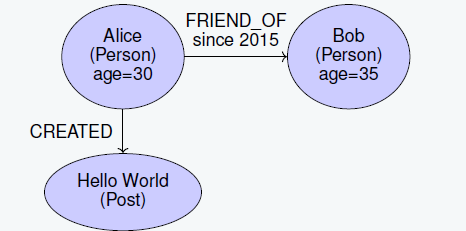
\includegraphics[width=\linewidth]{images/graph_db_instance.png}
        \caption{Instance}
    \end{minipage}
    \hfill
    \begin{minipage}[b]{0.48\linewidth}
        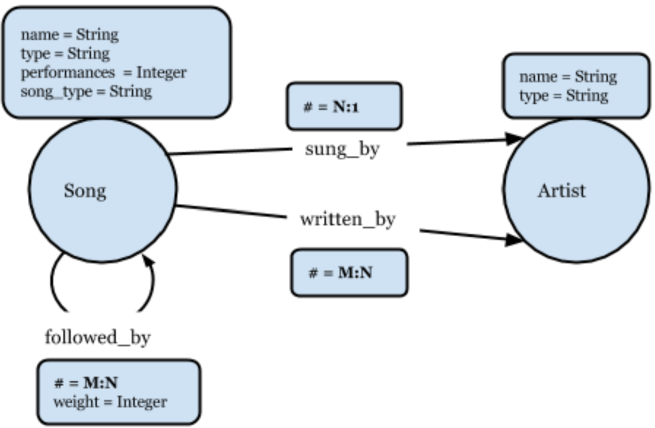
\includegraphics[width=\linewidth]{images/graph_db_schema.png}
        \caption{Schema}
    \end{minipage}
\end{figure}
\commandnote{
    Unlike relational databases, graph databases can be populated without prior specification of the schema!
}

\subsection*{Native vs Non-Native Storage}
\begin{itemize}
  \item \textbf{Native}: Index-free adjacency, fast for traversal
  \item \textbf{Non-Native}: Graph overlay on relational backend
\end{itemize}

\subsection*{ER to Graph Schema Transformation}
\begin{itemize}
  \item Entities \(\to\) Nodes
  \item Binary relations \(\to\) Edges
  \item N-ary relations \(\to\) Nodes with role-labeled edges
\end{itemize}

\minititle{Examples:}
\begin{figure}[H]
    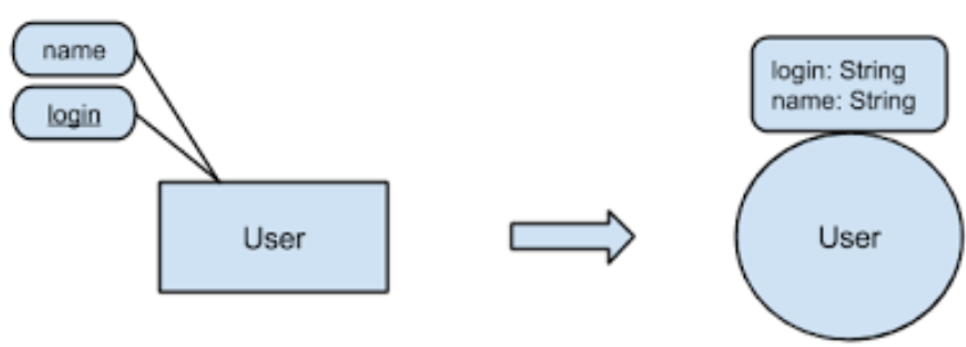
\includegraphics[width=0.4\linewidth]{images/1.png}
\end{figure}
    
\begin{figure}[H]
    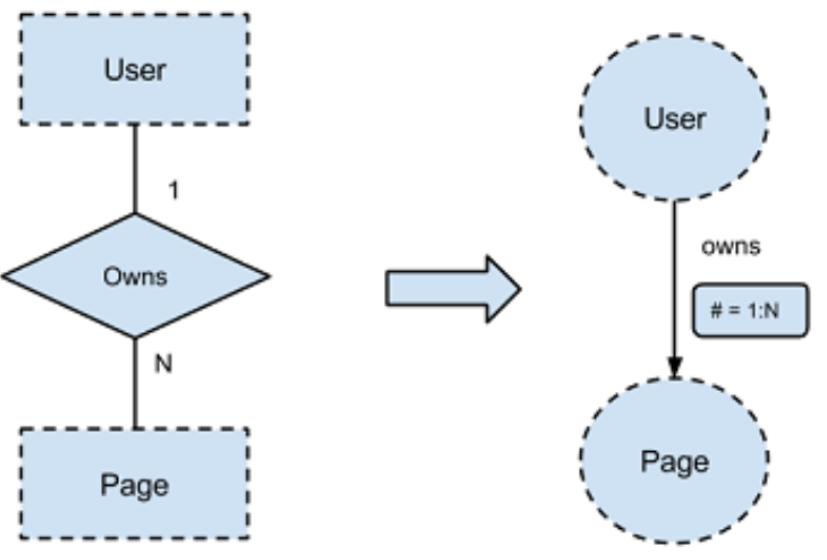
\includegraphics[width=0.4\linewidth]{images/2.png}
\end{figure}

\begin{figure}[H]
    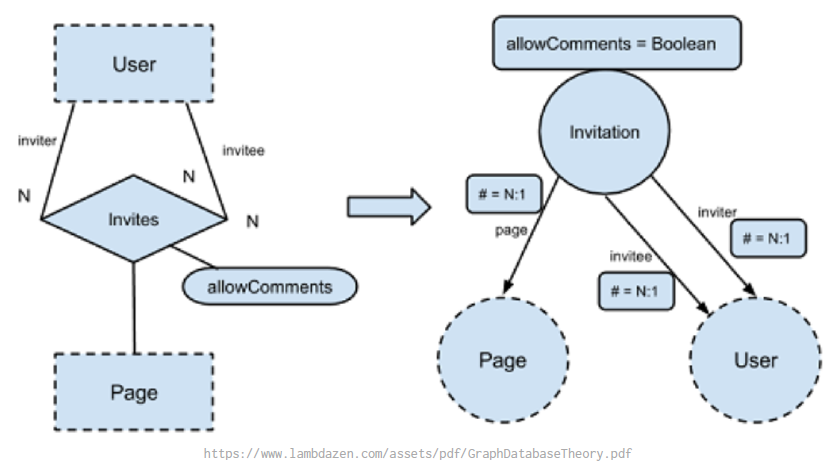
\includegraphics[width=0.4\linewidth]{images/3.png}
\end{figure}

\subsection*{Graph Schema Equivalence}
\mydef{Graph Universe}{
    The graph universe $U(S)$ of a graph schema $S$ is the infinite set of all graph instances of $S$
}

\mydef{Equivalent}{
    Two graph schemata $S$ and $\hat{S}$ are equivalent iff $\exists f. f:U(S)\to U(\hat{S})$
}


\subsection*{Graph Schema Transformation Rules}
\begin{itemize}
  \item \textbf{Renaming}: Change label/property names \textit{(schema-preserving)}
  \item \textbf{Reverse Edges}: Invert direction if no conflict exists
  \item \textbf{Property Displacement}: Move edge prop to node if look-across is 1
  \item \textbf{Specialization/Generalization}: Split or merge types by property predicates
  \item \textbf{Edge Promotion}: Turn edge into node with two new edges
  \item \textbf{Property Promotion}: Factor property set into a separate node
  \item \textbf{Multivalued Expansion}: Turn list-valued property into connected nodes
\end{itemize}

\minititle{Derived Vertex Types, Edge Types, and Properties}

Let $S$ be a graph schema and $U(S)$ the corresponding graph universe.

\begin{itemize}
    \item A vertex type $T$ is \emph{derived} in $S$ iff, for all graphs $G \in U(S)$, the graph $G$ can be uniquely reconstructed from $G - V_T$, where $V_T$ is the set of all vertices in $G$ with type $T$.
    
    \item An edge type $T$ is \emph{derived} in $S$ iff, for all graphs $G \in U(S)$, the graph $G$ can be uniquely reconstructed from $G - E_T$, where $E_T$ is the set of all edges in $G$ with type $T$.
    
    \item A vertex or edge property $P$ is \emph{derived} in $S$ iff, for all graphs $G \in U(S)$, the graph $G$ can be uniquely reconstructed from a graph $G'$ where the property $P$ has been deleted from all vertices and edges.
\end{itemize}

\minititle{General Rule To Simplify Graph Schemas}
Given a graph schema $S$, deleting a derived property or vertex/edge type yields an equivalent graph schema $\hat{S}$

\minititle{General Rule To Make Graph Schemas More Complex}
Given a graph schema $S$, adding a vertex type, edge type, or property $T$ such that $T$ is derived in $\hat{S} = S + T$ yields an equivalent graph schema $\hat{S}$

\subsection*{Cypher Query Language}
\mydef{Cypher}{Declarative graph query language used in Neo4j. Pattern-based, ASCII-art style.}

\minititle{Pattern Matching}
\texttt{MATCH (a:Person)-[:KNOWS]->(b) RETURN b.name}

\minititle{Core Constructs}
\begin{itemize}
  \item Node: \texttt{(p:Person \{name: 'Anna'\})}
  \item Edge: \texttt{[:KNOWS \{since: 2019\}]}
  \item Path: \texttt{(a)-[:KNOWS*1..3]-(b)} (1--3 undirected hops)
  \item Undirected Edge: \texttt{(a)-[:KNOWS]-(b)}
\end{itemize}

\minititle{Modifying Data}
\textbf{CREATE}
\begin{itemize}
  \item \texttt{CREATE (a:Person \{name: 'Bob'\})} -- new node
  \item \texttt{CREATE (a)-[:KNOWS]->(b)} -- new edge
\end{itemize}

\textbf{DELETE}
\begin{itemize}
  \item \texttt{DELETE a} -- only if a has no edges
  \item \texttt{DETACH DELETE a} -- delete node and connected edges
\end{itemize}

\textbf{SET}
\begin{itemize}
  \item \texttt{SET a.surname = 'Smith'} -- add or update property
  \item \texttt{SET a = \{name: 'X', age: 42\}} -- overwrite all properties
\end{itemize}

\subsection*{Schema Constraints in Cypher}
\begin{itemize}
  \item \textbf{Uniqueness}: \texttt{REQUIRE (n.p1, n.p2) IS UNIQUE}
  \item \textbf{Existence}: \texttt{REQUIRE n.prop IS NOT NULL}
  \item \textbf{Type}: \texttt{REQUIRE n.prop IS :: STRING}
  \item \textbf{Key}: \texttt{REQUIRE (n.p1, n.p2) IS NODE KEY}
\end{itemize}

\mydef{Example: Key Constraint}{
Ensure each Actor has a unique name combination: \\
\texttt{CREATE CONSTRAINT actor\_id FOR (a:Actor) REQUIRE (a.firstname, a.surname) IS NODE KEY}
}

\newpage
\section{Descriptive Statistics and Data Normalization}
\subsection*{Measures of Central Tendency}
\mydef{Mean}{
    $\mu = \frac{1}{n} \sum_{i=1}^n x_i$
}

\commandnote{Mean is best for symmetrical distributions without outliers}

\minititle{Optimization-Based Median}
In the context of Optimization, the median for $n$ numbers is a \textit{set-valued function} when $n$ is even and a \textit{single-valued function} when $n$ is odd. The function gives us the value or the set of values that minimizes the distance to all elements.
\[
\text{Median} = \displaystyle \min_{x} \sum_{i=1}^n | x-x_i |
\]

\textbf{Examples (odd):}
data: $\set{1,2,3,6,10}$
we want to minimize $f(x)= \sum | x - x_i |$
\begin{itemize}
    \item $f(1) = |1-1| + |1-2| + |1-3| + |1-6| + |1-10| = 0 + 1 + 2 + 5 + 9 = 17$
    \item $f(2) = |2-1| + |2-2| + |2-3| + |2-6| + |2-10| = 1 + 0 + 1 + 4 + 8 = 14$
    \item $f(3) = |3-1| + |3-2| + |3-3| + |3-6| + |3-10| = 2 + 1 + 0 + 3 + 7 = 13$
    \item $f(6) = |6-1| + |6-2| + |6-3| + |6-6| + |6-10| = 5 + 4 + 3 + 0 + 4 = 16$
    \item $f(10) = |10-1| + |10-2| + |10-3| + |10-6| + |10-10| = 9 + 8 + 7 + 4 + 0 = 28$
\end{itemize}
Hence, the minimum occurs at $x = 3$ with $f(3) = 13$. Since the number of data points is odd, the optimization-based median is \textbf{unique} and equal to the middle value in the sorted list: $\boxed{3}$.

\textbf{Examples (even):}
data: $\set{1,2,3,6}$
we want to minimize $f(x)= \sum | x - x_i |$
\begin{itemize}
    \item $f(1) = |1-1| + |1-2| + |1-3| + |1-6| = 0 + 1 + 2 + 5 = 8$
    \item $f(2) = |2-1| + |2-2| + |2-3| + |2-6| = 1 + 0 + 1 + 4 = 6$
    \item $f(3) = |3-1| + |3-2| + |3-3| + |3-6| = 2 + 1 + 0 + 3 = 6$
    \item $f(6) = |6-1| + |6-2| + |6-3| + |6-6| = 5 + 4 + 3 + 0 = 12$
\end{itemize}
We observe that $f(x)$ attains its minimum value of $6$ for any $x \in [2, 3]$. Since the number of data points is even, the optimization-based median is \textbf{set-valued}, and any value in the interval $\boxed{[2, 3]}$ minimizes the total absolute deviation.

\commandnote{
    The Optimization-Based Median can be computed using simple rules when the data is sorted in ascending order and indexed as $x_1, x_2, \dots, x_n$. If $n$ is odd, the median is the single value at index $i = \frac{n+1}{2}$ (i.e., the middle element). If $n$ is even, the median is any value in the interval $[x_{n/2},\, x_{ \frac{n}{2} + 1}]$.
}

\minititle{Statistical Median}
Conventually in statistics, the median is always one single value, therefore when $n$ is even, the median is calculated as $\frac{x_{\frac{n}{2}} + x_{\frac{n}{2}+1}}{2}$. and for odd we just use the middle value formula ($x_{\frac{n+1}{2}}$)

\textbf{Example:}
Data: $\{1, 4, 7, 9\}$

Here, $n = 4$ is even, so we compute:
\[
\text{median} = \frac{x_2 + x_3}{2} = \frac{4 + 7}{2} = \boxed{5.5}
\]

\commandnote{Median is preferred for skewed distributions or when outliers are present}

\mydef{Mode}{
    The most frequent value(s) in the dataset. $\text{mode} = \operatorname*{arg\,max}_{x} \left| \left\{ i \in \{1, \dots, n\} \mid x_i = x \right\} \right|$
}
\textbf{Example:}

Data: $\{2, 3, 5, 3, 8, 3, 2\}$

We compute the size of each set:
\begin{align*}
&\left|\left\{ i \mid x_i = 2 \right\}\right| = 2 \quad \text{(indices 1 and 7)} \\
&\left|\left\{ i \mid x_i = 3 \right\}\right| = 3 \quad \text{(indices 2, 4, and 6)} \\
&\left|\left\{ i \mid x_i = 5 \right\}\right| = 1 \quad \text{(index 3)} \\
&\left|\left\{ i \mid x_i = 8 \right\}\right| = 1 \quad \text{(index 5)}
\end{align*}

The maximum count is $3$, which occurs at $x = 3$.

\commandnote{Mode is useful for categorical data or to identify the most frequent value}

\minititle{Unimodal vs. Multimodal}
\begin{figure}[H]
    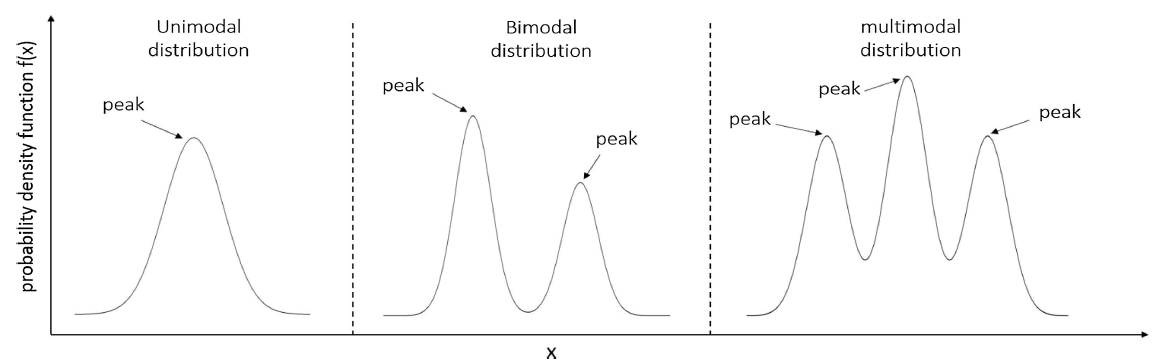
\includegraphics[width=0.5\linewidth]{images/unimodal_multimodal.png}
\end{figure}

\subsection*{Measures of Dispersion}
\mydef{Range}{
    The difference between the maximum and minimum values ($\displaystyle \max_{i} X_i \; - \; \min_{i} X_i$)
}
\commandnote{
    Range is best for a quick estimate of variability. However it is sensitive to outliers since it only considers extreme values
}

\mydef{IQR}{
    Interquartile Range (IQR) is the difference between the third quartile (Q3) and first quartile (Q1), measuring the spread of the middle 50\% of data ($Q_3 - Q_1$)
}
\commandnote{
    IQR is a robust measure of spread. It is useful when dealing with skewed distributions or outliers since it ignores extreme values
}

\mydef{Variance $\sigma^2$}{
    The average squared deviation from the mean. Calculated as $\sigma^2 = \frac{1}{n} \sum_{i=1}^n (X_i - \mu_X)^2$
}

\mydef{Unnormalized Variance (Total Variability)}{
    The raw sum of squares, called total sum of squares. $\text{TSS} = \sum_{i=1}^n (X_i - \mu_X)^2 = n \sigma_X^2$
}
\commandnote{
    Variance measures overall data dispersion. However, squaring emphasizes larger deviations, making it more sensitive to extreme values
}


\mydef{Standard Deviation $\sigma$}{
    The square root of variance ($\sqrt{\sigma^2}$), indicating the average deviation from the mean
}

\mydef{Unnormalized Standard Deviation}{
    $\hat{\sigma}_X=\sqrt{\text{TSS}} = \sqrt{\sum_{i=1}^n (X_i - \mu_X)^2} = \sqrt{n \sigma_X^2} = \sqrt{n}\sigma_X$
}
\commandnote{
    Standard Deviation is measured in the same unit as the data (more intuitive). It is used in many statistical methods like confidence intervals and hypothesis testing
}

\mydef{Covariance}{
    $\text{Cov}(X,Y) = \frac{1}{n} \sum_{i=1}^n (x_i - \mu_X)(y_i - \mu_Y)$
}

\mydef{Unnormalized Covariance}{
    $\text{Cov}_{unnormalized}(X,Y) = \sum_{i=1}^n (x_i - \mu_X)(y_i - \mu_Y) = n \text{Cov}(X,Y)$
}

\mydef{Coefficient of Variation (CV)}{
    relative measure of dispersion, calculated as the standard deviation divided by the mean ($\text{CV}=\frac{\sigma}{\mu} \times 100\%$)
}

\commandnote{
    CV is useful for comparing variability across datasets with different units or scales. Low CV indicates less relative variability and more consistency. High CV suggests greater dispersion relative to the mean
}

\textbf{Side Note: }Only use CV for data measured on a ratio scale, where quantity ratios and zeros are meaningful.

\mydef{Skewness}{
    Measures data asymmetry by relating the average cubed distances from the mean to the standard deviation. It is calculated as $\frac{\frac{1}{n}\sum_{i=1}^n (X_i - \mu)^3}{\sigma^3}$.
}

The Cubed distances from the mean preserve sign of distances, tend to cancel out for symmetric distributions.

\commandnote{
    Skewness close to zero: indicates a symmetric distribution (mean, median and mode are close). Positive skewness: suggests a longer right tail (mode $\leq$ median $\leq$ mean). Negative skewness: indicates a longer left tail (mode $\geq$ median $\geq$ mean)
}

\subsection*{Measures of Correlation}
\minititle{Pearson’s Correlation Coefficient}
Assume we have quantitative data points $X = \set{x_i \mid i \in [1\dots n]}$ and $Y = \set{y_i \mid i \in [1\dots n]}$. Pearson’s Correlation Coefficient ($r$) is defined as the covariance of $X$ and $Y$ divided by the product of their standard deviations:
\[
r = \frac{ \frac{1}{n} \sum_{i=1}^n (x_i - \mu_X)(y_i - \mu_Y)}{\sigma_X  \sigma_Y} = \frac{\text{Cov}(X,Y)}{\sqrt{\sigma_X^2}  \sqrt{\sigma_Y^2}} = \frac{\frac{1}{n} \sum_{i=1}^n (x_i - \mu_X)(y_i - \mu_Y)}{\sqrt{\frac{1}{n} \sum_{i=1}^n (X_i - \mu_X)^2} \sqrt{\frac{1}{n} \sum_{i=1}^n (y_i - \mu_Y)^2}} \quad \quad \boxed{r(X,Y) \in  [-1,1]}
\]
\begin{figure}[H]
    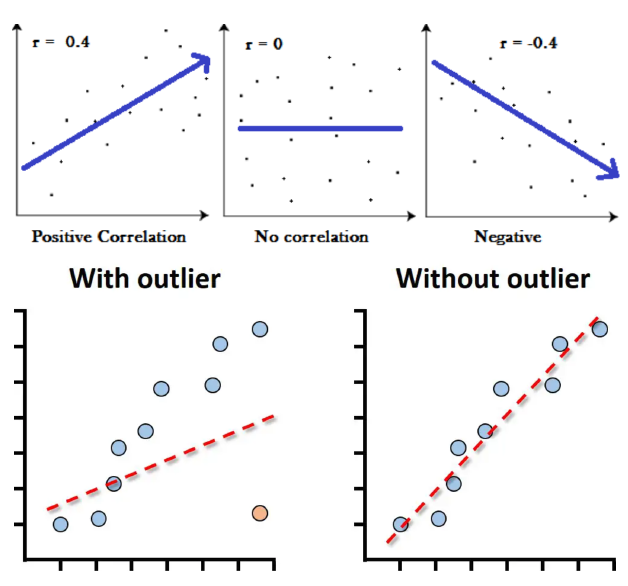
\includegraphics[width=0.3\linewidth]{images/pearson.png}
\end{figure}

\textbf{Unnormalized r:}
\[
\hat{r} = \frac{\text{Cov}_{unnormalized}(X,Y)}{\sqrt{\text{TSS}_X} \sqrt{\text{TSS}_Y}} = \frac{\sum_{i=1}^n (x_i - \mu_X)(y_i - \mu_Y)}{\sqrt{\sum_{i=1}^n (x_i - \mu_X)^2} \sqrt{\sum_{i=1}^n (y_i - \mu_Y)^2}}
\]

\mydef{OLS Regression}{
To find the line that best fits our data and explain how our $Y$ is linearly dependent on $X$, we find model parametes $\alpha$ and $\beta$ that minimize the sum of squared errors $\sum_{i=1}^n (y_i - \hat{y}_i)^2$ where $\hat{y_i} = \alpha x_i + \beta + \epsilon_i$
}
There is a \textit{closed-form} solution for this optimization problem and that is:
\[
\alpha = \frac{\text{Cov}_{unnormalized}(X,Y)}{\text{TSS}_X} = 
 \frac{\sum_{i=1}^n(x_i - \mu_X)(y_i - \mu_Y)}{\sum_{i=1}^n(x_i - \mu_X)^2}
\]

\[
= \frac{n \text{Cov}(X,Y)}{n \sigma_X^2} = \frac{\text{Cov}(X,Y)}{\sigma_X^2}
\]
Remember: $r = \frac{\text{Cov}(X,Y)}{\sigma_X  \sigma_Y}$. Meaning: $\text{Cov}(X,Y) = r \sigma_X  \sigma_Y$
\[
\alpha = \frac{r \sigma_X  \sigma_Y}{\sigma_X^2} = r\frac{\sigma_Y}{\sigma_X}
\]

\[
\beta = \mu_Y - \alpha \mu_X
\]

\mydef{Explained Variability}{
    Once we fit a line $\hat{y_i} = \alpha x_i + \beta + \epsilon$ we can calculate the explained variability. $\sum_{i=1}^n (\hat{y}_i - \mu_Y)^2$
}

\mydef{Coefficient of Determination ($R^2$)}{
    What fraction of the total variability in $Y$ is explained by our linear model. 
}
\[
    R^2 = \frac{\text{Explained Variability}}{\text{Total Variability}} = \frac{\sum_{i=1}^n (\hat{y}_i - \mu_Y)^2}{\sum_{i=1}^n (y_i - \mu_Y)^2} \qquad R^2 = 1 \to \text{perfect prediction}
\]

\[
\text{Remember: }
\hat{y}_i = \alpha x_i + \beta \text{ and } \mu_Y = \alpha \mu_X + \beta
\]

\[
R^2 = \frac{\sum_{i=1}^n (\alpha x_i + \beta - (\alpha \mu_X + \beta))^2}{\sum_{i=1}^n (y_i - \mu_Y)^2}
\]

\[
R^2 = \frac{\sum_{i=1}^n (\alpha x_i + \beta - \alpha \mu_X - \beta)^2}{\sum_{i=1}^n (y_i - \mu_Y)^2}
\]

\[
R^2 = \frac{\sum_{i=1}^n (\alpha x_i - \alpha \mu_X)^2}{\sum_{i=1}^n (y_i - \mu_Y)^2}
\]

\[
R^2 = \frac{\sum_{i=1}^n (\alpha (x_i - \mu_X))^2}{\sum_{i=1}^n (y_i - \mu_Y)^2}
\]

\[
R^2 = \frac{\alpha^2 \sum_{i=1}^n (x_i - \mu_X)^2}{\sum_{i=1}^n (y_i - \mu_Y)^2} = \frac{\alpha^2 \text{TSS}_X}{\text{TSS}_Y} = \alpha^2 \frac{n \sigma_X^2}{n \sigma_Y^2} = \frac{\alpha^2 \sigma_X^2}{\sigma_Y^2} 
\]

\[
\text{Remember: } \alpha = r\frac{\sigma_Y}{\sigma_X} \text{ Hence }\alpha^2 = r^2 \frac{\sigma_Y^2}{\sigma_X^2}
\]

\begin{align*}
R^2 &= \alpha^2 \frac{\sigma_X^2}{\sigma_Y^2} \\
&= r^2 \frac{\sigma_Y^2}{\sigma_X^2} \frac{\sigma_X^2}{\sigma_Y^2} \\
R^2 &= r^2
\end{align*}

\minititle{Spearman’s Rank Correlation Coefficient}
Because $r$ is sensitive to outliers and only suitable for linear relationships. We apply the Rank-Transformation trick to the data by the following steps:
\begin{enumerate}
    \item Transform data $X = \set{x_i \mid i \in [1\dots n]}$ and $Y = \set{y_i \mid i \in [1\dots n]}$ into fractional ranks $X^R = \set{x^R_i \mid i \in [1\dots n]}$ and $Y^R = \set{y^R_i \mid i \in [1\dots n]}$
    
        \begin{enumerate}
        \item For each $x_i$ collect set $J_i = \set{j \in [1 \dots n] \mid x_i = x_j}$ of indices $j$ of data points identical to $x_i$
        \item Sort the data in ascending order and store position $\pi_i$ of $x_i$ in sorted array (ordinal ranking)
        \item Compute fractional ranks as \textit{mean} of ordinal ranks of identical values:
        \[
        X_i^R = \frac{\sum_{i\in J_i} \pi_i}{|J_i|} = \frac{\text{min}_{j \in J_i} \pi_i + \text{max}_{j \in J_i} \pi_i}{2}
        \]
        \end{enumerate}
    \item Compute Spearman’s rank correlation coefficient as Pearson’s correlation coefficient ($r$) of rank-transformed data $X^R$ and $Y^R$
    \[
    \rho = r(X^R, Y^R) = 
    \frac{\sum_{i=1}^n (x_i^R - \mu_X^R)(y_i^R - \mu_Y^R)}
    {\sqrt{\sum_{i=1}^n (x_i^R - \mu_X^R)^2} \sqrt{\sum_{i=1}^n (y_i^R - \mu_Y^R)^2}}
    \]
\end{enumerate}
\commandnote{
    The mean of the ordinal ranks of elements in $J_i$ is equal to the mean of the minimum and maximum of these ordinal ranks
}

Assume we have data $[1,2,2,2,3]$ and their ordinal ranks $[1,2,3,4,5]$. We have $k=3$ tied elements starting from $r=2$, their ordinal ranks are $2,3,4$ which is $r, r+1, r+2$ and their mean is $\frac{r + (r+1)+ (r+2)}{k}$. The general formula for the mean is:
\[
    \frac{(r)+ (r+1)+ (r+2)+ \dots + (r+k-1)}{k}
\]

And the mean of the first and last ordinal ranks is $\frac{r + (r+k-1)}{2} = \frac{2r+k-1}{2} = \frac{2r}{2} + \frac{k-1}{2} = r (\frac{2}{2}) + \frac{k-1}{2} = r + \frac{k-1}{2}$

We want to prove the following equality:
\[
\frac{(r)+ (r+1)+ (r+2)+ \dots + (r+k-1)}{k} = r + \frac{k-1}{2}
\]
\begin{align*}
\frac{(r)+ (r+1)+ (r+2)+ \dots + (r+k-1)}{k} &= 
\frac{\sum_{i=0}^{k-1} r + i}{k} = \frac{1}{k}\sum_{i=0}^{k-1} r + i \\
\end{align*}
\[
\frac{1}{k}\sum_{i=0}^{k-1} r + i = \frac{1}{k} (\sum_{i=0}^{k-1} r + \sum_{i=0}^{k-1} i) \qquad \qquad \sum_{i=0}^{k-1} r \quad \text{evaluates to }kr
\]

\[
\sum_{i=0}^{k-1} i = \frac{k(k-1)}{2} \qquad \text{triangular numbers } (\sum_{i=1}^n i = 1+2+3+ \dots +n = \frac{n (n+1)}{2})
\]

\[
\frac{1}{k} (\sum_{i=0}^{k-1} r + \sum_{i=0}^{k-1} i) = 
\frac{1}{k} (kr + \frac{k(k-1)}{2}) =
\frac{kr}{k} +  \frac{k(k-1)}{2k} = 
r + \frac{k-1}{2}
\]
\minititle{Example:}
Let:
\[
X = [1,\ 1,\ 3,\ 5,\ 5,\ 5,\ 7], \quad
Y = [2,\ 2,\ 4,\ 6,\ 7,\ 6,\ 9]
\]

\begin{enumerate}
    \item \textbf{Rank-transform both $X$ and $Y$}

    \textbf{Step 1: Ordinal Ranks}

    \begin{itemize}
        \item Sorted $X$: $[1, 1, 3, 5, 5, 5, 7]$ → Ordinal ranks: $[1, 2, 3, 4, 5, 6, 7]$
        \item Sorted $Y$: $[2, 2, 4, 6, 6, 7, 9]$ → Ordinal ranks: $[1, 2, 3, 4, 5, 6, 7]$
    \end{itemize}

    \textbf{Step 2: Fractional Ranks}

    \begin{itemize}
        \item For $X$:
        \[
        \begin{aligned}
        x_1 = x_2 = 1 &\Rightarrow x_1^R = x_2^R = \frac{1 + 2}{2} = 1.5 \\
        x_3 = 3 &\Rightarrow x_3^R = 3 \\
        x_4 = x_5 = x_6 = 5 &\Rightarrow x_{4..6}^R = \frac{4 + 6}{2} = 5 \\
        x_7 = 7 &\Rightarrow x_7^R = 7
        \end{aligned}
        \]
        \item For $Y$:
        \[
        \begin{aligned}
        y_1 = y_2 = 2 &\Rightarrow y_1^R = y_2^R = \frac{1 + 2}{2} = 1.5 \\
        y_3 = 4 &\Rightarrow y_3^R = 3 \\
        y_4 = y_6 = 6 &\Rightarrow y_4^R = y_6^R = \frac{4 + 5}{2} = 4.5 \\
        y_5 = 7 &\Rightarrow y_5^R = 6 \\
        y_7 = 9 &\Rightarrow y_7^R = 7
        \end{aligned}
        \]
    \end{itemize}

    \textbf{Fractional Ranks:}

    \[
    X^R = [1.5,\ 1.5,\ 3,\ 5,\ 5,\ 5,\ 7]
    \quad
    Y^R = [1.5,\ 1.5,\ 3,\ 4.5,\ 6,\ 4.5,\ 7]
    \]

    \item \textbf{Compute Pearson $r$ on ranks}

    \begin{itemize}
        \item Mean ranks:
        \[
        \mu_X^R = \frac{1}{7}(1.5 + 1.5 + 3 + 5 + 5 + 5 + 7) = \frac{28}{7} = 4
        \]
        \[
        \mu_Y^R = \frac{1}{7}(1.5 + 1.5 + 3 + 4.5 + 6 + 4.5 + 7) = \frac{28}{7} = 4
        \]

        \item Numerator

        \[
        \sum (x_i^R - \mu_X^R)(y_i^R - \mu_Y^R) \approx 22.25
        \]
      
        \item Denominator
        \[
        \sqrt{\sum_{i=1}^n (x_i^R - \mu_X^R)^2} \sqrt{\sum_{i=1}^n (y_i^R - \mu_Y^R)^2}
         = \sqrt{25.5} \sqrt{27}
        \]
        \item Then:
       \[
        \rho = \frac{22.25}{\sqrt{25.5} \cdot \sqrt{27}} = \frac{22.25}{\sqrt{688.5}} \approx \frac{22.25}{26.24} \approx 0.848
        \]
    \end{itemize}
\end{enumerate}

\subsection*{Visualization}
\minititle{Box Plots}
\begin{figure}[H]
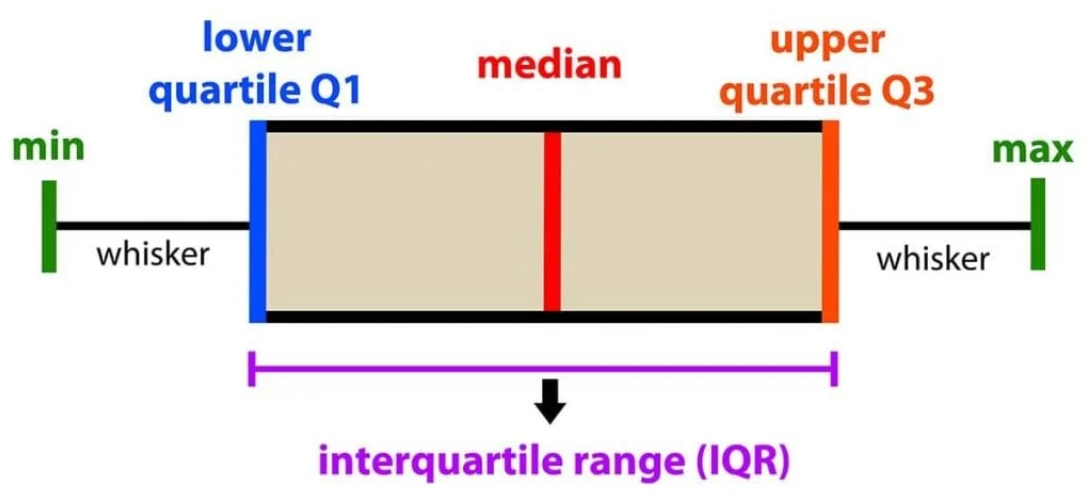
\includegraphics[width=0.4\linewidth]{images/boxplot.png}
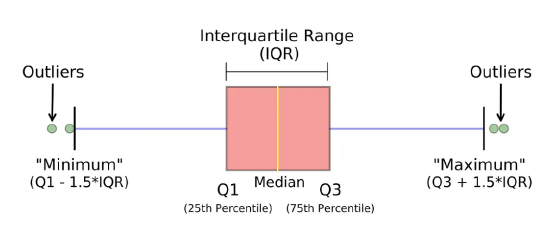
\includegraphics[width=0.4\linewidth]{images/boxplot2.png}
\end{figure}

\textbf{Use Case (Detecting Outliers):}
Given the sorted dataset:
\[
\text{data} = [10, 20, 30, 40, 50, 60, 70, 80, 90, 500], \quad n = 10
\]

To compute the 25th percentile using linear interpolation, we use the formula:
\[
\text{Position} = \frac{p}{100} \cdot (n - 1)
\]

Substituting \(p = 25\), we get:
\[
\text{Position} = \frac{25}{100} \cdot (10 - 1) = 0.25 \cdot 9 = 2.25
\]

This indicates that the 25th percentile lies 25\% of the way between the values at positions 2 and 3 (using zero-based indexing), which are:
\[
\text{data}[2] = 30, \quad \text{data}[3] = 40
\]

We linearly interpolate between these values:
\[
\text{25th percentile} = 30 + 0.25 \cdot (40 - 30) = 30 + 2.5 = 32.5
\]

Therefore, the 25th percentile of the dataset is:
\[
\boxed{Q1 = 32.5}
\]

For the 75th percentile:
Substituting \(p = 75\), we get:
\[
\text{Position} = \frac{75}{100} \cdot (10 - 1) = 0.75 \cdot 9 = 6.75
\]

This indicates that the 75th percentile lies 75\% of the way between the values at positions 6 and 7, which are:
\[
\text{data}[6] = 70, \quad \text{data}[7] = 80
\]

We linearly interpolate between these values:
\[
\text{75th percentile} = 70 + 0.75 \cdot (80 - 70) = 70 + 7.5 = 77.5
\]

Therefore, the 75th percentile of the dataset is:
\[
\boxed{Q3 = 77.5}
\]

Using Q1 and Q3, we can calculate $\text{IQR} = Q3 - Q1 = 77.5 - 32.5 = 45$

From that, we can calculate lower and upper bounds to detect outliers:
\[
\text{Lower Fence} = Q_1 - 1.5 \cdot \text{IQR} = 32.5 - 67.5 = -35
\]
\[
\text{Upper Fence} = Q_3 + 1.5 \cdot \text{IQR} = 77.5 + 67.5 = 145
\]

Min and Max (excluding outliers):
\[
\text{Min} = 10, \quad \text{Max} = 90
\]

\textbf{Outlier:} The value 500 exceeds the upper fence and is therefore an outlier.



\minititle{Scatter Plots}
\begin{figure}[H]
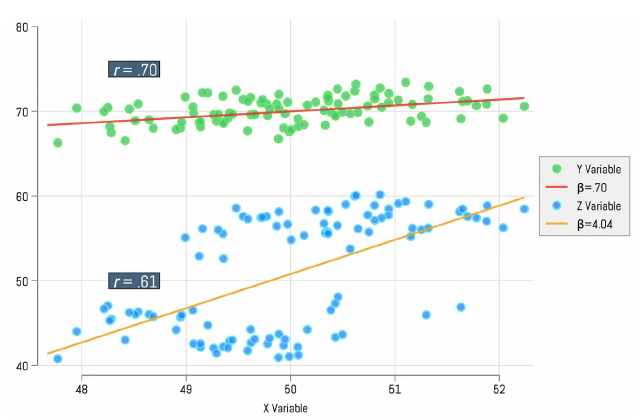
\includegraphics[width=0.5\linewidth]{images/scatterplot.png}
\end{figure}

\minititle{Heat Maps}
\begin{figure}[H]
    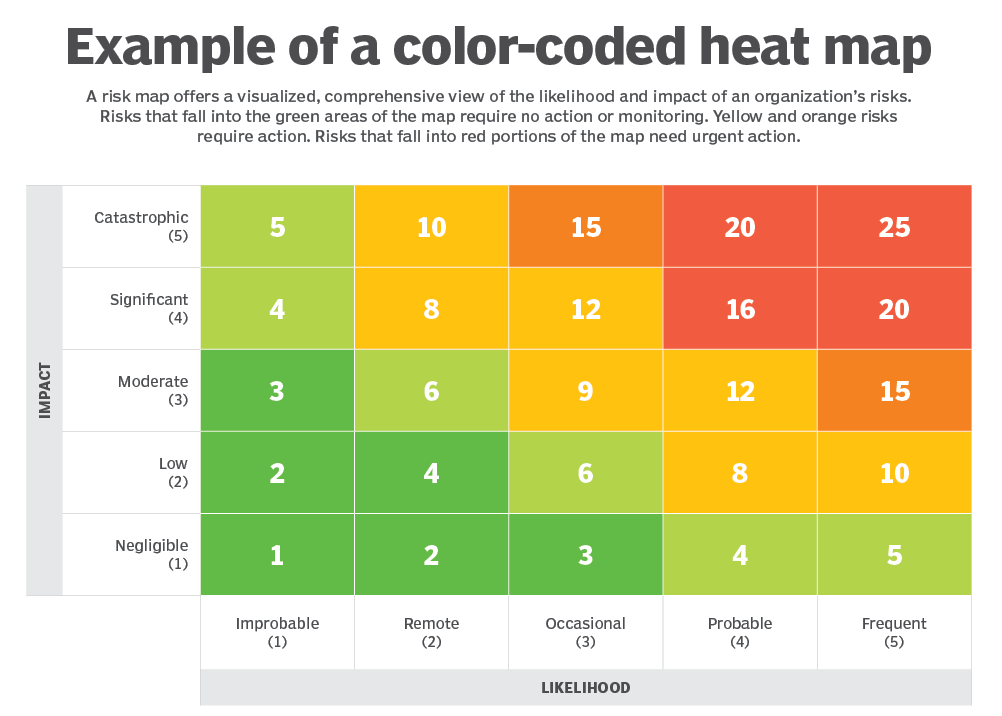
\includegraphics[width=0.5\linewidth]{images/heatmap.png}
\end{figure}

\minititle{Histograms and Bar Charts}
\begin{figure}[H]
    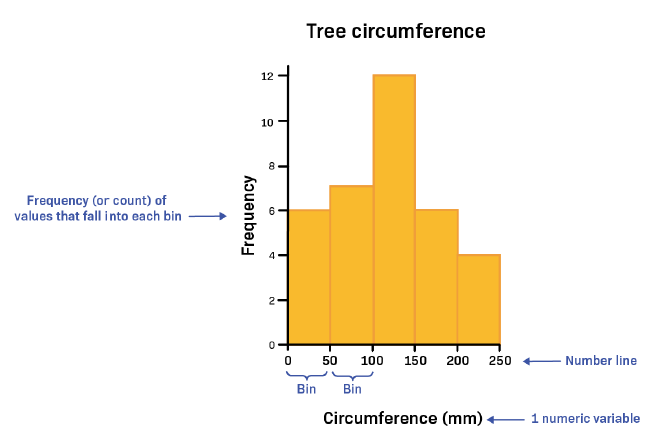
\includegraphics[width=0.48\linewidth]{images/histogram.png}
    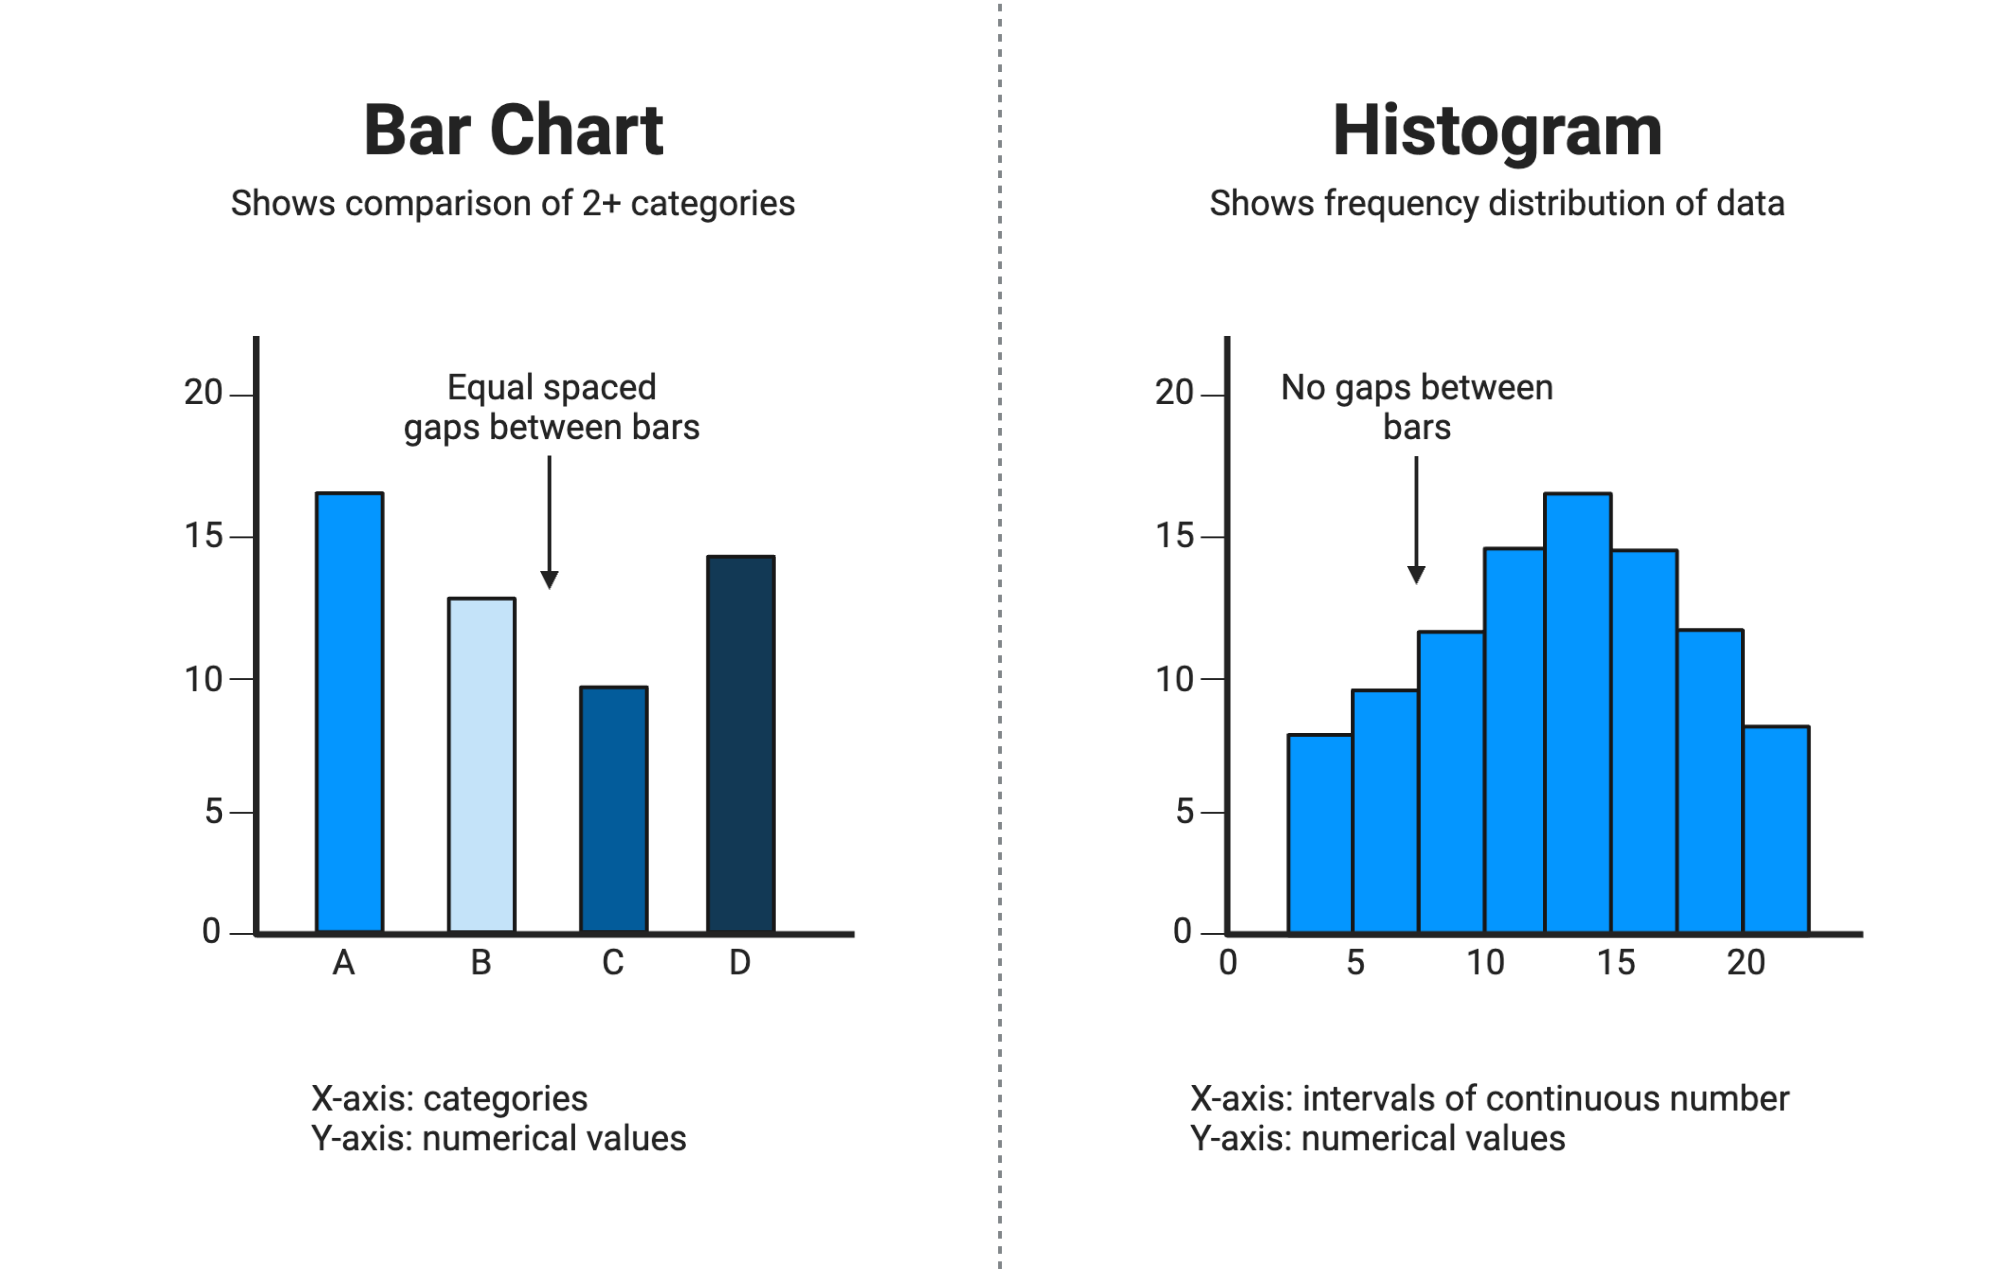
\includegraphics[width=0.48\linewidth]{images/histogram_vs_barchart.png}
\end{figure}

\minititle{KDE Plots}
\begin{itemize}
    \item Provides smooth estimate of the probability density function (PDF) from data, as a continuous alternative to a histogram.
    \item Each data point $x_i$ contributes a Gaussian $\mathcal{N}(x_i, h^2)$ to the total density. These are averaged to get an estimate of the full density
    \[
    f(x) = \frac{1}{nh} \sum_{i=1}^n \frac{1}{\sqrt{2 \pi}} e^{-\frac{(x-x_i)^2}{2h^2}}
    \]
    \item too small $h \to$ under-smoothed plot
    \item too high $h \to$ over-smoothed plot
\end{itemize}
\begin{figure}[H]
    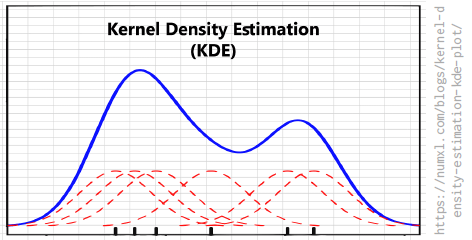
\includegraphics[width=0.5\linewidth]{images/kde.png}
\end{figure}

\text{Detect skewness from density plots:}
\begin{figure}[H]
    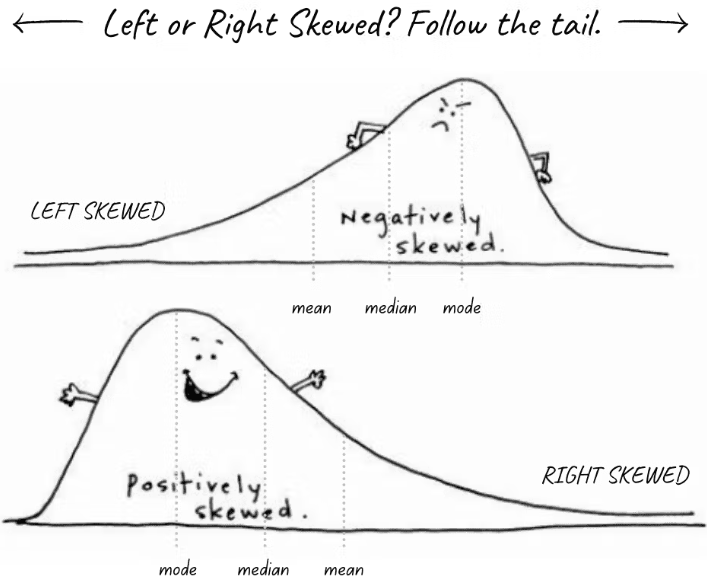
\includegraphics[width=0.3\linewidth]{images/skew.png}
\end{figure}
\minititle{Violin Plots}
A violin plot shows \textbf{summary statistics} \textit{(box plot)} and \textbf{full distribution} \textit{(KDE)}
\begin{figure}[H]
    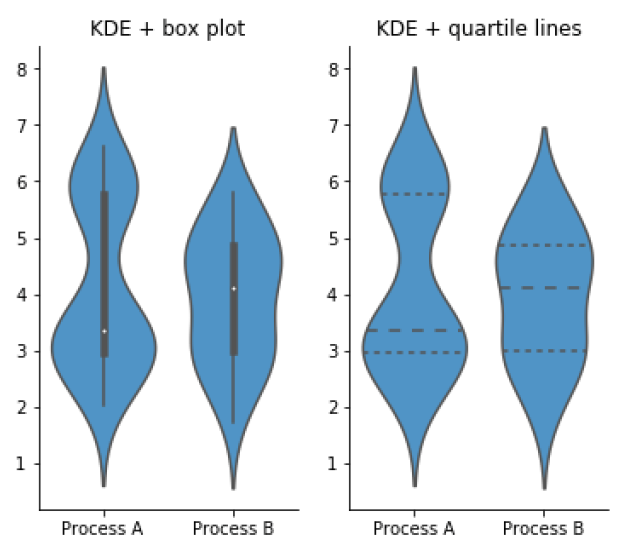
\includegraphics[width=0.3\linewidth]{images/violin.png}
\end{figure}

\subsection*{Normalization}
\minititle{Min-Max}
\begin{itemize}
    \item Preserves orders and scaling. Fixed range $[0,1]$ (Good for bounded data)
    \item Sensitive to outliers and does not generalize well
\end{itemize}
\[
\hat{x} = \frac{x-\text{min}}{\text{max} - \text{min}}
\]

\minititle{Z-Score}
Useful when data is not bounded. Handles outliers well. Normalized data have zero mean and standard deviation of one. Handles varying distributions.
\[
\hat{x} = \frac{x - \mu_X}{\sigma_X}
\]

\minititle{Robust Scaling}
More resistant to outliers (best for handling outliers). Works well with skewed and non-Gaussian data
\[
\hat{x} = \frac{x - \text{median}_X}{\text{IQR}_X}
\]

\minititle{Decimal Scaling}
Used when you want to avoid using min-max but still need a fixed range (Quick and dirty)
\[
\hat{x} = \frac{x}{10^k} \text{ where } k \text{ is the smallest natural number such that }\frac{x}{10^k} \in [-1,1] \forall x
\]

\minititle{Log Transformation}
\begin{itemize}
    \item Reduces skewness and improves normality. Stabilizes variance and Preserves order.
    \item Best for reducing skewness in rightskewed data.
    \item Not defined for negative values and can distort small values
\end{itemize}
\[
\hat{x} = \text{log}(x + 1)
\]

\minititle{What to choose?}
\begin{itemize}
    \item No one-size-fits-all solution: choose based on data properties and requirement analysis
    \item Consider preprocessing techniques before normalization
    \item Always visualize data before and after transformation
\end{itemize}

\textbf{Consider the Data Distribution}
\begin{itemize}
    \item If your data is \textit{right-skewed}, use log transformation
    \item If it is with outliers, use robust scaling
    \item If transformed data needed in fixed range, then min-max or decimal
    \item If your data is normality distributed, then use Z-scores
\end{itemize}

\newpage
\section{Distance and Similarity Measures}
\textbf{Matrix Multiplication }
$A = \begin{bmatrix}
a & b \\
c & d
\end{bmatrix}
\qquad
B = \begin{bmatrix}
e & f \\
g & h
\end{bmatrix}
\qquad
AB = \begin{bmatrix}
ae + bg & af + bh \\
ce + dg & cf + dh
\end{bmatrix}
$

\mydef{Symmetric}{
    A matrix $A$ is symmetric iff $A = A^T$. Or iff $A_{ij} = A_{ji} \quad \forall\, i,\, j$. \textbf{Example: }$
A = \begin{bmatrix}
2 & 5 \\
5 & 3
\end{bmatrix}
$
}

\mydef{Positive Definite (PD)}{
    A \textbf{symmetric matrix} $A$ is \textbf{positive definite} if, for every \textbf{nonzero} vector $x$, $x^T A x > 0$. Example:
}
Let
$
A = \begin{bmatrix}
2 & 0 \\
0 & 3
\end{bmatrix}
$
For any vector $x = \begin{bmatrix} a \\ b \end{bmatrix}$,
\[
x^T A x = \begin{bmatrix} a & b \end{bmatrix}
\begin{bmatrix} 2 & 0 \\ 0 & 3 \end{bmatrix}
\begin{bmatrix} a \\ b \end{bmatrix}
= \begin{bmatrix} a & b \end{bmatrix} \begin{bmatrix} 2a \\ 3b \end{bmatrix}
= 2a^2 + 3b^2
\]
For any $x \neq 0$, $2a^2 + 3b^2 > 0$, so $A$ is positive definite.


\mydef{Positive Semi-Definite (PSD)}{
    A \textbf{symmetric matrix} $A$ is \textbf{positive semi-definite} if, for \text{every vector} $x$, $x^T A x \geq 0$. Example:
}

Let $A = \begin{bmatrix}
1 & 0 \\
0 & 0
\end{bmatrix}
$
For any $x = \begin{bmatrix} a \\ b \end{bmatrix}$,
\[
x^T A x = \begin{bmatrix} a & b \end{bmatrix}
\begin{bmatrix} 1 & 0 \\ 0 & 0 \end{bmatrix}
\begin{bmatrix} a \\ b \end{bmatrix}
= \begin{bmatrix} a & b \end{bmatrix}
\begin{bmatrix} a \\ 0 \end{bmatrix}
= a^2
\]
$a^2 \geq 0$ always. So $A$ is positive semi-definite, but not positive definite.

\mydef{Gram Matrix}{
    Given vectors $x_1, x_2, \dots, x_n$ in $\mathbb{R}^d$, the \textbf{Gram matrix} $G$ is the $n \times n$ matrix whose entries are all possible dot products:
$
G_{ij} = x_i^T x_j
$
for $i, j = 1, \ldots, n$. Example:
}

Let
$
x_1 = \begin{bmatrix} 1 \\ 2 \end{bmatrix}, \quad
x_2 = \begin{bmatrix} 3 \\ 4 \end{bmatrix}
$

Compute all dot products:
\begin{align*}
x_1^T x_1 &= 1 \times 1 + 2 \times 2 = 1 + 4 = 5 \\
x_1^T x_2 &= 1 \times 3 + 2 \times 4 = 3 + 8 = 11 \\
x_2^T x_1 &= 3 \times 1 + 4 \times 2 = 3 + 8 = 11 \\
x_2^T x_2 &= 3 \times 3 + 4 \times 4 = 9 + 16 = 25 \\
\end{align*}
Thus, the Gram matrix is
\[
G = \begin{bmatrix}
x_1^T x_1 & x_1^T x_2 \\
x_2^T x_1 & x_2^T x_2
\end{bmatrix}
=
\begin{bmatrix}
5 & 11 \\
11 & 25
\end{bmatrix}
\]
Note that, considering the vectors matrix $X = \begin{bmatrix}
1 & 3 \\
2 & 4
\end{bmatrix}$. The Gram matrix is $X^T X$
\[
X^T = \begin{bmatrix}
1 & 2 \\
3 & 4
\end{bmatrix}
\qquad
X^T X =
\begin{bmatrix}
1 & 2 \\
3 & 4
\end{bmatrix}
\begin{bmatrix}
1 & 3 \\
2 & 4
\end{bmatrix}
=
\begin{bmatrix}
5 & 11 \\
11 & 25
\end{bmatrix}
\]

Properties of the Gram Matrix:
\begin{itemize}
    \item Symmetric: $G_{ij} = G_{ji}$.
    \item Positive semi-definite (PSD): For any vector $c$,
    $
    c^T G c \geq 0
    $
\end{itemize}



\mydef{Distance Measures}{
    Quantify how far apart two objects are. \textit{Properties: }symmetrical, non-negative, triangle inequality (direct path is at least as short as any detour), etc.
}

\mydef{Similarity Measures}{
    Quantify how similar or alike two objects are. \textit{Properties: }symmetrical and ranges from 0 (completely different) to 1 (completely alike)
}

\mydef{Metrics}{
    Let $X$ be a set of data objects, $x,y,z \in X$. A \textbf{metric} is a distance function $d: X \times X \to \mathbb{R}$ that satisfies:
}
\begin{enumerate}
    \item Non-negativity: $d(x,y) \geq  0 \quad \forall x,y \in X$
    \item Identity of indiscernibles: $d(x,y) = 0 \Leftrightarrow x = y$
    \item Symmetry: $d(x,y) = d(y,x)$
    \item Triangle inequality: $d(x,z) \leq d(x,y) + d(y,z)$
\end{enumerate}

\mydef{Pseudometrics}{
    Same as \textbf{metrics} but allow zero distance between different objects
}
\begin{enumerate}
    \item Non-negativity: $d(x,y) \geq  0 \quad \forall x,y \in X$
    \item $d(x,x) = 0$ and it is possible that $d(x,y) = 0 \quad x \neq y$
    \item Symmetry: $d(x,y) = d(y,x)$
    \item Triangle inequality: $d(x,z) \leq d(x,y) + d(y,z)$
\end{enumerate}
Example (Pseudometrics): 
\[
d(x, y) =
  \begin{cases}
    0 & \text{if } \operatorname{lowercase}(x) = \operatorname{lowercase}(y) \\
    1 & \text{otherwise}
  \end{cases} \qquad d(\text{Apple}, \text{apple}) = 0
\]

\mydef{Quasimetrics}{
    A quasimetric is a distance function that \textit{relaxes} the symmetry requirement of a \textbf{metric} 
}
\begin{enumerate}
    \item Non-negativity: $d(x,y) \geq  0 \quad \forall x,y \in X$
    \item Identity of indiscernibles: $d(x,y) = 0 \Leftrightarrow x = y$
    \item Triangle inequality: $d(x,z) \leq d(x,y) + d(y,z)$
\end{enumerate}

\minititle{From Distance to Similarity and Vice Versa}
\mydef{Linear Scaling}{
    $d(x,y) = 1 - \frac{s(x,y)}{s_{\text{max}}} \qquad s(x,y) = 1 - \frac{d(x,y)}{d_{\text{max}}}$
}
Example: $d(\text{cat}, \text{cat}) = 0 \qquad s(\text{cat}, \text{cat}) = 1$
\commandnote{
    Preserves relative differences in distances. Requires normalization of distances. Not suitable for unbounded distances.
}

\mydef{Reciprocal transformation}{
    $s(x,y) = \frac{1}{1 + d(x,y)}$
}
Example: $d(\text{cat}, \text{dog}) = 2 \qquad s(\text{cat}, \text{dog}) = 0.33$
\commandnote{
    Keeps values bounded between 0 and 1. Works well when small distances should lead to high similarity. Sensitive to large distances, as similarity first decays quickly and then slowly.
}

\mydef{Exponential decay}{
    $s(x,y) = e^{- \lambda d(x,y)} \quad \lambda=\frac{1}{\mu_d}$
}
Example:
\begin{itemize}
    \item $d(\text{cat}, \text{cat}) = 0$
    \item $d(\text{cat}, \text{dog}) = 2$
    \item $d(\text{cat}, \text{lion}) = 4$
    \item $\mu_d = 2 \qquad \lambda = 0.5$
    \item $s(\text{cat}, \text{cat}) = e^{- \lambda d(x,y)} = e^{0} = 1$
    \item $s(\text{cat}, \text{dog}) = e^{- \lambda d(x,y)} = e^{-1} = 0.368$
    \item $s(\text{cat}, \text{lion}) = e^{- \lambda d(x,y)} = e^{-2} = 0.135$
\end{itemize}

\commandnote{
    Smoothly decreases similarity with increasing distance. Handles large distances better than reciprocal transformation. Requires tuning $\lambda$ and can be unintuitive when distances vary widely.
}

\mydef{Dot Product}{
    For vectors $x,y \in \mathbb{R}^n \quad |x|=|y|$ their dot product is given by $x . y = \sum_{i=1}^n x_i y_i$
}
\begin{itemize}
    \item Dot product between two vectors measure their \textbf{alignment}
    \item It ranges from $- \infty$ to $+ \infty$
    \item If $x$ and $y$ point in the same direction, then $x . y > 0$
    \item If $x$ and $y$ point in opposite directions, then $x . y < 0$
    \item If they are \textbf{orthogonal (perpendicular)}, then $x . y = 0$
\end{itemize}

\textbf{Remember (The Norms):}

A norm on a vector space is a function $\|\cdot\|$ that satisfies:
\begin{itemize}
    \item Positive Definiteness: $\|x\| \geq 0$ with equality iff $x=0$
    \item Homogeneity: $\| \lambda x\| = |\lambda| \|x\| $
    \item Triangle Inequality: $\|x+y\| \leq \|x\| + \|y\|$
\end{itemize}
\textbf{Most Common Norms: $L_1, L_2, L_p, L_{\infty}$}

$\|x\|_1 = \sum_{i=1}^n |x_i| \quad$
$\|x\|_2 = \left( \sum_{i=1}^n |x_i|^2 \right)^{1/2} \quad$
$\|x\|_p = \left( \sum_{i=1}^n |x_i|^p \right)^{1/p} \quad$
$\|x\|_{\infty} = \text{max}_i |x_i|$

\textbf{Note: }a norm \textit{induces} a \textbf{metric} $d(x,y) = \|x-y\|$ which satisfies:
\begin{itemize}
    \item $d(x,y) \leq 0$ and $d(x,y)=0$ iff $x=y$
    \item $d(x,y) = d(y,x)$
    \item $d(x,y) \leq d(x,y) + d(y,z)$
\end{itemize}

\mydef{Cosine Similarity}{
    A normalized version of the \textbf{dot product}. It measures the angle between two vectors regardless their magnitude. $s_C (x,y) = cos(\theta_{x,y}) = \frac{x.y}{\left\lVert x\right\rVert_2 \left\lVert y \right\rVert_2}$
}

\commandnote{
    Cosine similarity ranges from $-1$ (opposite direction) to $1$ (same direction), if they are orthogonal then $0$
}

\mydef{Cosine Distance}{
    $d_{\text{cosine}}(x,y) = 1 - s_C(x,y)$. Range is $[0,2]$ (unintuitive)
}
\commandnote{Cosine Distance does not satisfy the triangle inequality}

\mydef{Angular Distance}{
    $d_{\text{angular}}(x,y) = \frac{\theta_{x,y}}{\pi} = \frac{\text{cos}^{-1} (s_C(x,y))}{\pi}$. Range is $[0,1]$
}
\commandnote{
    Angular Distance satisfies the triangle inequality
}

\commandnote{
    When comparing vectors of different magnitudes, neither cosine nor angular distance always respect the "identity of indiscernibles" axiom, meaning two different vectors can sometimes have zero distance under these measures if one is a scaled version of the other (colinear).
}

\textbf{Example: Cosine Distance Does Not Satisfy Identity of Indiscernibles}

Let $x = [1,\,2]$ and $y = [2,\,4]$ (note $y = 2x$):

\[
\|x\|_2 = \sqrt{1^2 + 2^2} = \sqrt{5}
\]
\[
\|y\|_2 = \sqrt{2^2 + 4^2} = \sqrt{20}
\]
\[
x \cdot y = 1 \cdot 2 + 2 \cdot 4 = 10
\]
\[
s_C(x, y) = \frac{10}{\sqrt{5}\sqrt{20}} = \frac{10}{10} = 1
\]
\[
d_{\text{cosine}}(x, y) = 1 - 1 = 0
\]

But $x \neq y$, so the identity of indiscernibles is not satisfied.

\textbf{Example: Cosine Distance Violates the Triangle Inequality}

Let $x = [1,\,0]$, $y = [0,\,1]$, and $z = [1,\,1]$:

\[
d_{\text{cosine}}(x, y) = 1 - 0 = 1
\]

\[
x \cdot z = 1 \cdot 1 + 0 \cdot 1 = 1
\]
\[
\|z\|_2 = \sqrt{1^2 + 1^2} = \sqrt{2}
\]
\[
s_C(x, z) = \frac{1}{1 \cdot \sqrt{2}} = \frac{1}{\sqrt{2}} \approx 0.707
\]
\[
d_{\text{cosine}}(x, z) = 1 - 0.707 = 0.293
\]
Similarly, $d_{\text{cosine}}(y, z) \approx 0.293$

But:
\[
1 \nleq 0.293 + 0.293 = 0.586
\]
So the triangle inequality is violated.

\textbf{Example: Angular Distance Does Not Satisfy Identity of Indiscernibles}

Let $x = [1,\,2]$ and $y = [2,\,4]$:

\[
s_C(x, y) = 1
\]
\[
d_{\text{angular}}(x, y) = \frac{\arccos(1)}{\pi} = \frac{0}{\pi} = 0
\]

But $x \neq y$, so the identity of indiscernibles is not satisfied.

\mydef{Euclidean (L2) Distance}{
    $d_{\text{Euclidean}}(x,y) = \sqrt{\sum_{i=1}^n (x_i - y_i)^2}$ (L2 Norm of the difference vector)
}

It is the most commonly used distance measure in vector spaces. It represents the straight-line (geometric) distance between two points in Euclidean space.
\commandnote{
    Euclidean Distances satisfies all four metric properties. It is widely used in machine learning, clustering, nearest-neighbor search, etc., due to its intuitive geometric interpretation.
}

\mydef{Manhattan (L1) Distance (taxicab)}{
    $d_{\text{Manhattan}}(x,y) = \sum_{i=1}^n |x_i - y_i|$ (L1 Norm of the difference vector)
}

It measures the shortest path between points if movement is restricted to axis-aligned steps (like navigating city blocks in a grid). It satisfies all four metric properties. It is often used in ML and clustering when axis-aligned movement makes sense.

\mydef{Minkowski ($L_p$) Distance}{
    $d_p (x,y) = \left( \sum_{i=1}^n |x_i - y_i|^p \right)^{1/p}$
}

\commandnote{
    The larger $p$, the bigger the impact of the dimensions with the larger differences on the overall distance. The Minkowski distance satisfies all metric properties $\forall p \geq 1$
}

\mydef{Chebyshev ($L_{\infty}$) Distance}{
    $d_{\infty}(x,y) = \text{max}_i |x_i - y_i|$
}
\begin{itemize}
    \item Measures the greatest absolute difference between any coordinate of two vectors
    \item It is the limit case of the Minkowski distance as $p \to \infty$
    \item Useful for scenarios where only the largest coordinate difference matters
    \item The unit ball (set of points at distance 1) under Chebyshev distance is a square in 2D
\end{itemize}

\minititle{Remember: Unit Ball}
For a given norm (distance function) $\|\cdot\|$, the unit ball is the set of all points (vectors) whose distance from the origin is less than or equal to one. Formally, in $\mathbb{R}^n$: $B = \set{x \in \mathbb{R}^n \mid \|x\| \leq 1}$. For example, consider $\mathbb{R}^2$ and L2 Norm, $B$ is the set of points $(x_1,x_2)$ such that $\sqrt{(x_1)^2 + (x_2)^2} \leq 1$, i.e. $x_1^2 + x_2^2 \leq 1$.

Remember, the circle of radius $r$ is the set of points $(x_1,x_2)$ such that $x_1^2 + x_2^2 = r^2$. Hence, unit ball of L2 norm is a circle.

For a point $(x_1,x_2)$ the Chebyshev norm is $\text{max}(|x_1|,|x_2|)$. The unit ball for Chebyshev norm are the points $(x_1,x_2)$ where $\text{max}(|x_1|,|x_2|) \leq 1$. Hence, unit ball of $L_{\infty}$ is a square.

For $L1$, the unit ball is all points $(x_1, x_2)$ such that $|x_1| + |x_2| \leq 1$. Hence, the unit ball is a diamond for $L1$.


\minititle{Excursion}
Let's pick a vector and compute two different norms:

Let $x = (3, 4)$ in $\mathbb{R}^2$.
\[
\|x\|_1 = |3| + |4| = 7
\]
\[
\|x\|_2 = \sqrt{3^2 + 4^2} = \sqrt{9 + 16} = \sqrt{25} = 5
\]

Let's try another two vectors:

Let $y = (1, 0)$:
\[
\|y\|_1 = |1| + |0| = 1
\]
\[
\|y\|_2 = \sqrt{1^2 + 0^2} = 1
\]

Let $z = (1, 1)$:
\[
\|z\|_1 = |1| + |1| = 2
\]
\[
\|z\|_2 = \sqrt{1^2 + 1^2} = \sqrt{2} \approx 1.414
\]

Compare the Norms:
\begin{center}
\begin{tabular}{|c|c|c|c|c|}
\hline
\textbf{Vector} & $\|x\|_1$ & $\|x\|_2$ & $\|x\|_2 \leq \|x\|_1$ & $\|x\|_1 \leq \sqrt{2}\|x\|_2$ \\
\hline
$(3,4)$   & $7$   & $5$       & $5 \leq 7$     & $7 \leq 7.07$ \\
$(1,0)$   & $1$   & $1$       & $1 \leq 1$     & $1 \leq 1.41$ \\
$(1,1)$   & $2$   & $1.414$   & $1.414 \leq 2$ & $2 \leq 2$ \\
\hline
\end{tabular}
\end{center}

In all cases,
\[
\|x\|_2 \leq \|x\|_1 \leq \sqrt{2}\|x\|_2
\]

The General Pattern: For any vector $x$ in $\mathbb{R}^2$,
$
\|x\|_2 \leq \|x\|_1 \leq \sqrt{2}\|x\|_2
$.
For $x$ in $\mathbb{R}^n$,
$
\|x\|_2 \leq \|x\|_1 \leq \sqrt{n}\|x\|_2
$

In the general equivalence of norms, $C_1$ and $C_2$ are the constants making the inequalities true for all vectors:
\[
C_1 \|x\|_2 \leq \|x\|_1 \leq C_2\|x\|_2
\]

For $L_1$ and $L_2$ in $\mathbb{R}^2$, these are $C_1 = 1$ and $C_2 = \sqrt{2}$:
\[
1 \cdot \|x\|_2 \leq \|x\|_1 \leq \sqrt{2}\cdot\|x\|_2
\]


\textbf{Theorem: }For any two norms $\|\cdot\|_a$ and $\|\cdot\|_b$ on a finite-dimensional vector space, there exist constants $C_1, C_2 > 0$ such that, for all vectors $x$:
\[
C_1 \|x\|_a \leq \|x\|_b \leq C_2 \|x\|_a
\]


\minititle{Correlation-Based Similarity}
\begin{itemize}
    \item Pearson $r$ quantities similarity as degree of linear correlation
    \item Spearman $\rho$ quantities similarity as monotonicity of $x$ w.r.t $y$
    \item $\text{corr}(x,y) \in [-1,1]$
\end{itemize}

\mydef{Kernel Function}{
    A function $k(x, \bar{x})$ that computes the similarity between two input vectors $x$ and $\bar{x}$ and satisfies the following properties
}
\begin{enumerate}
    \item Symmetry: $k(x, \bar{x}) = k(\bar{x}, x)$
    \item Positive semi-definiteness: For any finite set $\set{x_1, \cdots, x_n}$ of vectors, the Gram matrix $K=(K_{ij}) \in \mathbb{R}^{n \times n}$ with entries $K_{ij}=k(x_i, x_j)$ is positive semi-definite (PSD), i.e. satisfies
    \[
    c^T Kc = \sum_{i=1}^{n} \sum_{j=1}^{n} c_i c_j k(x_i, x_j) \leq 0
    \]
    for all vectors of coefficients $c = (c_i) \in \mathbb{R}^n$
\end{enumerate}
\commandnote{
    The definition of a kernel does not require that $k$ is non-negative.
}

\mydef{Linear Kernel}{
    The simplest form of kernel (dot product similarity). $k(x, \bar{x}) = x \cdot \bar{x} = x^T \bar{x}$
}

Example: consider  
$
x = \begin{bmatrix} 1 \\ 2 \end{bmatrix}, \quad
\bar{x} = \begin{bmatrix} 3 \\ 4 \end{bmatrix}
$
Then $k(x, \bar{x}) = x^T \bar{x} = 1 \cdot 3 + 2 \cdot 4 = 3 + 8 = 11$

Proof that linear kernel is PSD:

For input vectors $x_1, x_2, \cdots, x_n$ our vectors matrix is $X = [x_1, x_2, \cdots, x_n]$ and the Gram matrix $K = X^T X$ (as shown previously)

For any vector $c$, we have $c^T K c = c^T X^T X c = (Xc)^T (Xc) = \|Xc\|_2^2 \geq 0 \quad \forall c$

\mydef{Gaussian (RBF) Kernel}{
    The Gaussian (radial basis function) kernel is the most widely used kernel in the ML field. $k(x, \bar{x}) = exp(-\frac{\|x - \bar{x}\|_2^2}{2 \sigma^2})$
}
\begin{itemize}
    \item small $\sigma \to$ kernel is more sensitive to distance between vectors 
    \item large $\sigma \to$ kernel is less sensitive to distance between vectors 
\end{itemize}

\mydef{Polynomial Kernel}{
    $k(x, \bar{x}) = (x^T \bar{x} + c)^d$. Where $d \geq 1$ is the degree. If $d=1$, the kernel captures linear relationships between the variables, if $d=2$, the kernel captures quadratic relationships, and so on. 
}
\commandnote{
    The larger the constant $c \geq 0$ the smoother the similarity landscape (small differences get swallowed by $c$)
}
Example: let $c=1$ and $d=2$, and assume we have 1D data $x,y \in \mathbb{R}$ then $k(x,y) = (xy + 1)^2 = x^2y^2 + 2xy + 1$

\textbf{Notice that }$x^2y^2 + 2xy + 1$ is the result of dot product between two feature vectors $\phi(x) = [x^2 , \sqrt{2} x, 1]$ and $\phi(y) = [y^2 , \sqrt{2} y, 1]$

Which means that the kernel is \textit{implicitly} mapping our original 1D data $(x,y)$ into a 3D space. i.e., we can instead of transforming all data into higher dimensions, we just use the kernel function which gives us inner product result as if we had transformed.
\begin{itemize}
    \item A linear kernel only detects linear alignment between data points
    \item A Polynomial kernel defines similarity in a much richer way: it says two inputs are similar if their higher-order features are similar, not just their values.
\end{itemize}

\mydef{Mercer’s Theorem}{
    if $k$ is a symmetric and PSD kernel function, then there exists a feature map $\phi$ into a higher-dimensional space $D$ (possibly $\infty$) such that $k(x,y) = \phi(x) \cdot \phi(y)$
}

\commandnote{
    In these higher-dimensional spaces, patterns may be detectable that are impossible or difficult to individuate in the original feature spaces.
}

\mydef{Kernel Trick}{
    A method in machine learning that enables algorithms which depend only on inner products between data points to be generalized to nonlinear feature spaces.
}

\commandnote{
    The kernel trick allows algorithms to operate in high- or infinite-dimensional feature spaces at the computational cost of operating in the original space, thereby enabling them to learn nonlinear patterns while remaining scalable.
}

Applications of the Kernel Trick in Machine Learning:
\begin{itemize}
    \item Support vector machines (SVMs): Supervised ML approach that implicitly fits separating hyperplanes in the higher-dimensional spaces.
    \item Kernelized perceptron: Another supervised ML approach that uses the kernel trick to learn non-linear decision boundaries.
    \item Kernel principal component analysis (kernel PCA): An extension of PCA that uses kernel functions to perform non-linear dimensionality reduction. It implicitly maps the data to a higher-dimensional space and then performs PCA in that space, allowing for the extraction of non-linear principal components.
    \item Kernelized clustering (e.g., k-means): Clustering methods that use the kernel trick to implicitly compute distances in the higher-dimensional space, allowing for the identification of non-linear clusters in the original data space.
\end{itemize}

\mydef{Edit Distances}{
    Ways to measure how different two structured objects are, typically strings, trees, or graphs.
}
\begin{itemize}
    \item You define a set of basic operations that can “edit” one object into another. \textit{Examples for strings: }insert a character, delete a character, substitute one character for another.
    \item Each operation has a cost (often 1 for each, but could be different).
    \item The edit distance between two objects $S$ and $T$ is the minimum total cost needed to turn $S$ into $T$ by a sequence of allowed operations.
\end{itemize}

Edit distances always respect the triangle inequality. If you know a way to turn $A$ into $B$ with cost $d(A,B)$, and a way to turn $B$ into $C$ with $d(B,C)$, then you could do both sequences of edits to turn $A$ into $C$ at a total cost $d(A,B) + d(B,C)$

Edit distances are generally not symmetric (Quasimetrics). The cost to edit $A$ into $B$ is not always the same as the cost to edit $B$ into $A$.

\mydef{Levenshtein Distance (metric)}{
    An edit distance for strings, defined as minimum number of single-character insertions, deletions, or substitutions needed to transform a source string $a$ into a target string $b$.
}
\[
\begin{array}{ll}
\textbf{Base Cases:} \\
\quad \text{lev}(a, "") = |a| \\
\quad \text{lev}("", b) = |b| \\[1em]
\textbf{Recursive Cases:} \\
\quad \text{lev}(a, b) =
  \begin{cases}
    \text{lev}(\text{tail}(a), \text{tail}(b)) & \text{if } \text{head}(a) = \text{head}(b) \\
    1 + \min\left\{
      \begin{array}{l}
        \text{lev}(\text{tail}(a), b) \\
        \text{lev}(a, \text{tail}(b)) \\
        \text{lev}(\text{tail}(a), \text{tail}(b))
      \end{array}
    \right. & \text{if } \text{head}(a) \neq \text{head}(b)
  \end{cases}
\end{array}
\]

Example:
\begin{align*}
\text{lev}(\text{"kit"}, \text{"cat"}) 
    &= \text{lev}(\text{"ki"}, \text{"ca"}) && \text{(heads: 't' = 't')} \\[1em]
\text{lev}(\text{"ki"}, \text{"ca"})
    &= 1 + \min \left\{
        \begin{array}{l}
            \text{lev}(\text{"k"}, \text{"ca"}) \\
            \text{lev}(\text{"ki"}, \text{"c"}) \\
            \text{lev}(\text{"k"}, \text{"c"})
        \end{array}
    \right. && \text{(heads: 'i' $\neq$ 'a')} \\[1em]
\text{lev}(\text{"k"}, \text{"ca"})
    &= 1 + \min \left\{
        \begin{array}{l}
            \text{lev}(\text{""}, \text{"ca"}) = 2 \\
            \text{lev}(\text{"k"}, \text{"c"}) = 1 \\
            \text{lev}(\text{""}, \text{"c"}) = 1
        \end{array}
    \right. (1 + \min\{1,1,0\}) \\[1em]
\text{lev}(\text{"ki"}, \text{"c"})
    &= 1 + \min \left\{
        \begin{array}{l}
            \text{lev}(\text{"k"}, \text{"c"}) = 1 \\
            \text{lev}(\text{"ki"}, \text{""}) = 2 \\
            \text{lev}(\text{"k"}, \text{""}) = 1
        \end{array}
    \right. \\[1em]
\text{lev}(\text{"k"}, \text{"c"})
    &= 1 + \min \left\{
        \begin{array}{l}
            \text{lev}(\text{""}, \text{"c"}) = 1 \\
            \text{lev}(\text{"k"}, \text{""}) = 1 \\
            \text{lev}(\text{""}, \text{""}) = 0
        \end{array}
    \right. \\[1em]
\end{align*}
Finally,
\begin{align*}
\text{lev}(\text{"ki"}, \text{"ca"})
    &= 1 + \min\{2,2,1\} = 1 + 1 = 2 \\[1em]
\text{lev}(\text{"kit"}, \text{"cat"})
    &= \text{lev}(\text{"ki"}, \text{"ca"}) = 2
\end{align*}

\mydef{Graph Edit Distance (GED)}{
    Given two graphs $G_1$ and $G_2$, $\text{GED}(G_1, G_2)$ is minimum cost of a sequence of edit operations that transform $G_1$ into a graph $\bar{G}_2$ that is \textbf{isomorphic} to $G_2$
}

\mydef{GED Edit Operations}{
    There are six elementary edit operations: Insertions of isolated nodes, deletions of isolated nodes, attribute substitutions for nodes, deletions of edges, insertions of edges between existing nodes, attribute substitutions for edges.
}

\commandnote{
    If "identity" means "isomorphism", then GED satisfies all pseudometric axioms. If "identity" means exact equality, then GED would be a metric.
}

\mydef{Shortest-Path Distance}{
    Let $G=\langle V,E \rangle$ be a graph, and let $w: E \to \mathbb{R}_{\geq 0}$ assign a non-negative weight (cost) to each edge. The shortest-path distance from node $u$ to $v \in V$ is: $d_G(u,v) = \text{min}_P \sum_{e \in P} w(e)$
}

In other words: The shortest-path distance between two nodes is the smallest possible total cost to travel from $u$ to $v$ along the edges of the graph.

\commandnote{
    In undirected graphs with symmetric edge costs, Shortest-path distance is a metric. In directed graphs or graphs with asymmetric edge costs, Shortest-path distance is a quasimetric.
}

\minititle{Linkage Distances for Clusters of Data Objects}
Consider we have a set of data objects $V$ that are grouped into $n$ clusters $\set{C_i, \cdots, C_n}$. And we also have a distance measure between individual objects $u,v \in V$ defined as $d_V : V \times V \to \mathbb{R}$.

We want to define a distance measure between \textbf{clusters} ($d(C_i, C_j)$)

\mydef{Linkage Distances}{
    Ways to aggregate (combine) the distances between all pairs of points in two clusters, in order to get a single distance value between the clusters themselves.
}

\mydef{Single Linkage}{
    $d_{SL}(C_i, C_j) = \text{min} \set{d_V(u,v) \mid (u,v) \in C_i \times C_j}$
}

For all possible pairs of points $(u,v)$ where $u \in C_i$ and $v \in C_j$ compute the distance $d_V(u,v)$ and take the smallest of these values. This is the minimum distance between the two clusters.

\mydef{Complete Linkage}{
    $d_{CL}(C_i, C_j) = \text{max} \set{d_V(u,v) \mid (u,v) \in C_i \times C_j}$ (maximum distance)
}

\mydef{Average Linkage}{
    $d_{AL}(C_i, C_j) = (|C_i| \cdot |C_j|)^{-1} \sum_{u \in C_i} \sum_{v \in C_j} d_V(u,v)$ (mean distance)
}
i.e. for all possible pairs $(u,v)$, sum all the distance and divide by number of all possible pairs.

\minititle{Sets Similarity and Distance}
\mydef{Jaccard Similarity}{
    For sets $A,B$, the Jaccard similarity is given by $J(A,B) = \frac{|A \cap B|}{|A \cup B|} \qquad \text{range} \to [0,1]$
}

\mydef{Jaccard Distance (metric)}{
   $d_J(A,B) = 1 - \frac{|A \cap B|}{|A \cup B|}$
}

\mydef{Sørensen-Dice Similarity}{
    $S(A,B) = \frac{2 |A \cap B|}{|A| + |B|}$. It is never smaller than the Jaccard index, $S(A,B) \geq J(A,B)$
}

\mydef{Sørensen-Dice Distance}{
    $d_S(A,B) = 1 - \frac{2 |A \cap B|}{|A| + |B|}$
}

\commandnote{
    The Sørensen-Dice “distance” fails the triangle inequality, so it is not a metric.
}

Proof by example:

Let:
\[
A = \{1\}, \quad B = \{1,2\}, \quad C = \{2\}
\]

Compute the Sørensen-Dice similarity for each pair:
\[
S(A,B) = \frac{2|A \cap B|}{|A| + |B|} = \frac{2 \cdot 1}{1 + 2} = \frac{2}{3}
\]
\[
S(B,C) = \frac{2|B \cap C|}{|B| + |C|} = \frac{2 \cdot 1}{2 + 1} = \frac{2}{3}
\]
\[
S(A,C) = \frac{2|A \cap C|}{|A| + |C|} = \frac{2 \cdot 0}{1 + 1} = 0
\]

Compute the corresponding distances:
\[
d_S(A, B) = 1 - S(A,B) = 1 - \frac{2}{3} = \frac{1}{3}
\]
\[
d_S(B, C) = 1 - S(B,C) = 1 - \frac{2}{3} = \frac{1}{3}
\]
\[
d_S(A, C) = 1 - S(A,C) = 1 - 0 = 1
\]

Sum the distances for the triangle inequality:
\[
d_S(A, B) + d_S(B, C) = \frac{1}{3} + \frac{1}{3} = \frac{2}{3}
\]
But:
\[
d_S(A, C) = 1 > \frac{2}{3} = d_S(A, B) + d_S(B, C)
\]

\minititle{Binary Data}
\mydef{Iverson bracket}{$[\text{True}] = 1$ and $[\text{False}] = 0$}

\mydef{Hamming Distance (metric)}{
    Quantifies the bit-wise difference between two binary arrays of the same size. For two binary arrays $A,B \in \set{0,1}^n$ it is defined as $\text{HD}(A,B) = \frac{1}{n} \sum_{i=1}^n [A_i \neq B_i]$
}

\end{document}

